

This chapter details the controller design and implementation in simulation and experiments. First, the control layout is detailed. Then, the model-based controller is detailed which comprises the systems Jacobian. Subsequently, the pressure controller is detailed which is used alongside the model-based controller. Before implementing the controller, the simulation model is compared to a quasi-static experimental analysis. Then, a closed-loop step response is considered to tune the controller in simulation. Subsequently, the performance of this controller is analyzed for a reference trajectory. Next, the experimental case is considered. The experimental setup is presented, where the hardware, sensory devices and communication is detailed. Also, the design of digital filters is explained which are used for data acquisition. Furthermore, the experimental tuning procedure is detailed. Then, the closed-loop step response is analyzed. Lastly, the results of a reference tracking problem conducted on the experimental setup are presented.



\section{Controller design}
\label{chap4a}

\subsection{Control layout}

Figure \ref{fig4:controllayout} shows the schematic overview of the soft robot's control layout. This control architecture is detailed starting with the end-effector's reference position vector $r_{set}$ containing the desired Cartesian $x$ and $y$ coordinate. This means that for position control the (coupled) rotation of the manipulator is omitted to avoid over constraining the system. Based on the estimated position through measurements $r_{est}$ in the Cartesian plane, position error vector $e_r$ can be determined. This error is injected into the model-based controller. This control law incorporates the current manipulator configuration through inverse kinematics. Based on the current configuration and position error, a control input $\nu_{set}$ is calculated. This control input can be viewed as a moment and force necessary to bend and elongate the soft robot. With the inverse of matrix $H$, the desired input force and moment can be converted to a reference pressure $p_{set}$. This vector contains the reference pressure for each bellow. The difference between measured pressure $p$ and the reference pressure is defined as the pressure error $e_p$. Based on this pressure error, the pressure controller determines the Volt input to the air pumps. The change in pressure affects position and orientation as perceived by the vision system and inertial measurement unit (IMU), respectively. The measured Cartesian coordinates of the end-effector and rotation allow calculation of the modal coordinates through inverse kinematics. These determined modal coordinates are subsequently used to update the model-based controller and calculate the new position error. 


\begin{figure}[H]
    \centering
    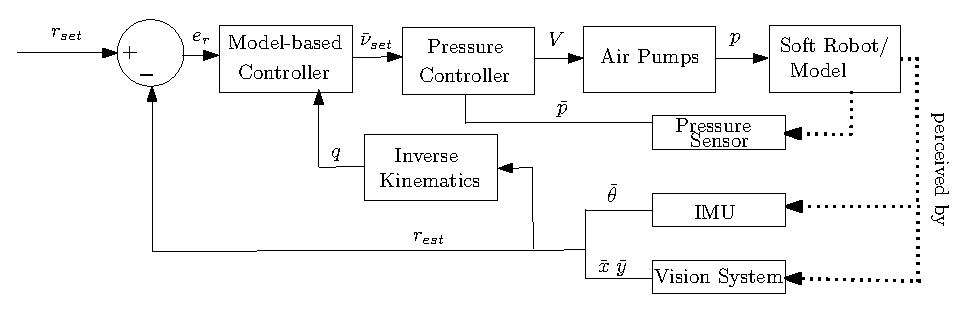
\includegraphics[width = \textwidth]{Figures/Chapter4/ControlschemeActualwithPump.eps}
    \caption{Control layout of the model-based controller accompanied by a low-level pressure controller.}
    \label{fig4:controllayout}
\end{figure}


\subsection{Jacobian model-based controller}


For controlling the soft robot, a model-based controller is proposed based on the system's Jacobian matrix. As mentioned in Chapter \ref{chapter1}, Jacobian control has readily been applied to the field of soft robotics. In this work, a Jacobian controller is implemented based on \cite{MOOSAVIAN20071226}. The latter work states that a computed torque controller can be approximated by a more straightforward control law involving the Jacobian transpose. This approximation holds if ``high enough" control gains are used. The work of \cite{MOOSAVIAN20071226} demonstrates this with a Jacobian PD controller. The control law that will be implemented is slightly altered. Since a PD controller has no integrator action, the steady-state error cannot be reduced. Furthermore, due to the high intrinsic damping present in soft robots, a differential action (i.e. $K_d \dot{e}$) is deemed not necessary to ensure a smooth transient. Therefore, a Jacobian PI controller will be implemented. The control law can then be formulated as,


\begin{equation}
    \nu_{set}(t) = \begin{bmatrix}J_c(\sigma,t)\end{bmatrix}_1^\top \Big(K_p e_r + K_i \int_0^t e_r \hspace{2pt} ds \Big) \hspace{10pt} \text{with} \hspace{10pt} e_r = r_{set}-r_{est}, 
    \label{eq:tau}
\end{equation}

where $\nu_{set}(t)$ is the desired control input, as calculated by the controller. Furthermore, the proportional-integrator structure can be directly observed. The diagonal gain matrices $K_p$ and $K_i$ both  $ \in \mathbb{R}^{2\times 2}$ contain proportional and integrator gains, respectively. The proportional gain matrix $K_p$ penalizes proportional to the position error, whereas the integrator gain matrix $K_i$ contributes to the sum of the error over time. The position error $e_r \in \mathbb{R}^2$ is defined as the difference between reference position vector $r_{set}$ and the estimated position vector in the (x,y)-plane $r_{est}$. The Jacobian is determined by (\ref{eq2:J}) following a first-order approximation, as shown in Chapter \ref{chap2}. Since only the position in (x,y)-plane is considered, not the entire Jacobian of dimension $3 \times 2$ is used. Only the entries mapping modal coordinate position to Cartesian position are used. This corresponds to the second and third row of the Jacobian, which will be defined as $[J_c]_1$. Due to its space dependency, the Jacobian is updated in real-time based on the actual kinematic configuration of the actuator. Based on the measured position and angle, the modal coordinates can be calculated through inverse kinematics. The simplified inverse kinematics are detailed in Appendix \ref{app4}.

Since the controller has a PI structure, oscillations in the control signal are not reduced as there is no derivative action in the control law. A derivative action could have easily been included based on numerical differentiation. However, this method often results in erroneous velocity estimated due to the presence of noise. The origin of the noise originates from position measurement which, through inverse kinematics, also affects the calculation of the Jacobian. Additionally, the vision system makes use of a discretized pixel grid, resulting in a discretized estimated position if not filtered. Instead of using a derivative action, a low-pass filter is added to the controller to reduce quick input changes. The discretized low-pass filter is given as,

\begin{equation}
\bar{\nu}_{set,k} = \zeta \nu_{set,k} + (1-\zeta)\bar{\nu}_{set,k-1}
\label{eq4:lowpass}
\end{equation}

where $\zeta$ with $ 0 < \zeta \leq 1$ is a weighing factor defining the relative importance between new input $\nu_{set,k}$ and previous input $\bar{\nu}_{set,k-1}$. A relatively high value of $\zeta$ increases the cut-off frequency, resulting in minimal noise reduction. A low value for $\zeta$ suppresses more frequencies but increases the input delays in the system, which can potentially cause stability problems. 


\subsection{Pressure controller}


The actual system does not allow to induce forces and moments directly. Therefore the set control input $\nu_{set}$ should be mapped to some reference pressure. This can be achieved by the mapping matrix as presented in Chapter \ref{chap3}. Recall that this positive-definite mapping matrix maps pressure to forces and moments. Therefore, its inverse can be used to map desired input force and moment to pressure. Based on the desired control input, a reference pressure can be formulated as,

\begin{equation}
    p_{set} = H^{-1}\bar{\nu}_{set},
\end{equation}


where vector $p_{set} \in \mathbb{R}^2$ contains the reference pressure for each bellow. To track this pressure reference a second controller is necessary. This low-level controller calculates the input voltage to the air pumps. A standard PI-controller is deemed sufficient to track the reference pressure. Therefore the control law is can be described by,

\begin{equation}
    V = K_{pp}e_p + K_{ip} \int_0^t e_p \hspace{2pt} ds \hspace{10pt} \text{with} \hspace{10pt} e_p = p_{set} - p,
\end{equation}

where $V \in \mathbb{R}^2$ is the input voltage based on the pressure error $e_p$. The proportional action is based on diagonal gain matrix $K_{pp} \in \mathbb{R}^{2\times 2}$, whereas the integral action is calculated by $K_{ip} \in \mathbb{R}^{2\times 2}$.





%%%%%%%%%%%%%
%%%%%%%%%%%%%%
%%%%%%%%%%%%
%%%%%%%%%%%




\section{Simulation and Experimental testing}
\label{chap4b}

\subsection{Dynamic model testing}
\label{subsecDMt}


To test the dynamic model, the model's response is compared to a measured response of the actual setup. To this end, the model and actual system are subjected to equivalent initial conditions and input. For a stable system, a free oscillation is preferred. This allows isolating the soft robot dynamics from the pump dynamics as the latter are not excited. However, such a free oscillation can not be induced on the physical setup. An initial curvature or elongation can be induced, although not being perfectly in-plane. This slight out-of-plane initial condition causes the soft to oscillate out-of-plane, making the observed response nugatory for parameter estimation.


Another method to perform a parameter estimation is comparing the model and experimental response subjected to an identical input signal. A significant limitation of this method is the involved pump dynamics. The dynamics of the pumps are slow compared to those of the soft robot i.e. $|\dot{q}|<< 1$ and $|\Ddot{q}|<< 1 $. Therefore, the mass and damping properties of the system will be hard to identify using this method. However, this method is suitable to conclude on the modelled stiffness properties. Since the FEM analysis is conducted on a manipulator with thinner walls, the actual stiffness is expected to deviate from the modelled stiffness. It is expected that the soft robot used for experiments is stiffer for both elongation and curvature. 

This experiment aims to find a linear scaling factor to scale the modelled non-linear stiffness to the actual stiffness. Since the accelerations and velocities are small the quasi-static modelled system can be expressed as,

\begin{equation}
   \underbrace{M(q) \Ddot{q}}_{\approx 0} + \underbrace{D \dot{q}}_{\approx 0} + K(q) q = Hp,
\end{equation}

where, for a steady state pressure, the modal coordinates only depend on the actual soft robot stiffness. It is assumed that the actual stiffnesses can be formulated as $K_{exp}(q) = G K(q) \hspace{4pt} \forall \hspace{2pt} q \in \mathcal{Q}$, with $G \in \mathbb{R}^{2\times 2}$ a diagonal matrix to tune the modeled stiffness and $\mathcal{Q} \subset \mathbb{R}$ the configuration space of the soft robot. Under the assumption that the measured pressure can be well described by a first-order model, the optimization to find $G$ can be formulated as, 


\begin{equation}
\begin{split}
    \underset{G}{\text{minimize}}& \sum_{k=0}^{N_{samples}} || q_{exp}(t_k) - q_{sim}(t_k)||  \\
    \text{s.t.} \hspace{10pt} & G K(q_{sim}) q_{sim} = Hp_{sim}
    \end{split}
    \label{eq5:optalpha}
\end{equation}

where $q_{exp}(t_k)$ are the experimentally obtained modal coordinates at sample instant $t_k$, and the $q_{sim}(t_k)$ the modal coordinates in simulation. Furthermore, $t_0 = 0$ and $t_{N_{samples}} = T$. Recall the force mapping $H$ as given in Chapter \ref{chap3}. The simulated pressure is described by $p_{sim}$. The input to the air pumps is chosen as,

\begin{equation}
    V_1 =
\begin{cases}
0 & 0 < t < 2\\
V & 2 \leq t < 22\\
0 & 22 \leq t < 122\\
V & 122 \leq t < 142\\
0 & 142 \leq t < 180\\
\end{cases} \hspace{30pt} \text{and} \hspace{30pt}      V_2 =
\begin{cases}
0 & 0 \leq t < 82\\
V & 62 \leq t < 82\\
0 & 82 \leq t < 122\\
V & 122 \leq t < 142\\
0 & 142 \leq t < 180\\
\end{cases} ,
\end{equation}

where the two step inputs between 2 and 22 and 42 and 62 seconds cause the soft robot to bend in a positive and negative direction, respectively. Between 142 and 162 seconds, an equal Volt input to both air pumps is supplied to induce an elongation. For this analysis, it was opted to use Volt step inputs as for such input accurate pressure models can be derived. This is beneficial when optimizing for $G$, as errors in modal coordinates are minimized when a valid pressure model is used. The analysis is repeated for Volt steps of 7, 9 and 11 Volts, respectively. For each air pump and Volt input, the attained experimental pressure is fit to a first-order linear model. This is the same model as used in Chapter \ref{chap3}.

The measured modal coordinates and results of the fitted stiffness are presented in Figure \ref{fig5:elong} and Figure \ref{fig5:kappa} for elongation and curvature, respectively. Instead of optimizing (\ref{eq5:optalpha}), the linear scaling for the stiffness curves has been obtained by iteratively running the dynamic model. Based on the outcomes of the steady-state elongation and curvature, $G$ is fitted. Initially, the optimization algorithm of (\ref{eq5:optalpha}) was utilized to find the scaling factors. However, the heavy computations resulted in exceptionally long simulation times. Therefore, this method was preferred, although being less accurate. Eventually, $G$ was found to be equal to $G = \text{diag}([3.125,3])$. This implies that the modelled stiffness is around a factor 3 lower compared to the actual stiffness. This result is logical, the soft robot model used for FEM analysis has thinner walls, attributing to less stiff yet more porous bellows. The experiments are carried out on a soft robot with thicker walls and therefore is stiffer. The mass of the system is equal to $33.2$ grams. The damping properties are chosen as $D = \text{diag}([4\cdot 10^{-5},2.5\cdot 10^{-2}])$. Furthermore, Figure \ref{fig5:p1} and \ref{fig5:p2} show the measured and simulated pressure. The pressure model describes the pressure for a curvature accurately. During the elongation, occurring between 120 and 140 seconds, the pressure model shows some deviation. Also, notice that the pumps do not reach an equal steady-state pressure for equivalent Volt input. This also results in curvature during the elongation phase, as can be seen in Figure \ref{fig5:kappa}. This behaviour is caused by the deterioration of the pumps after extended use. 

\begin{figure}[H] 
    \begin{minipage}[b]{0.49\linewidth}
     \centering
    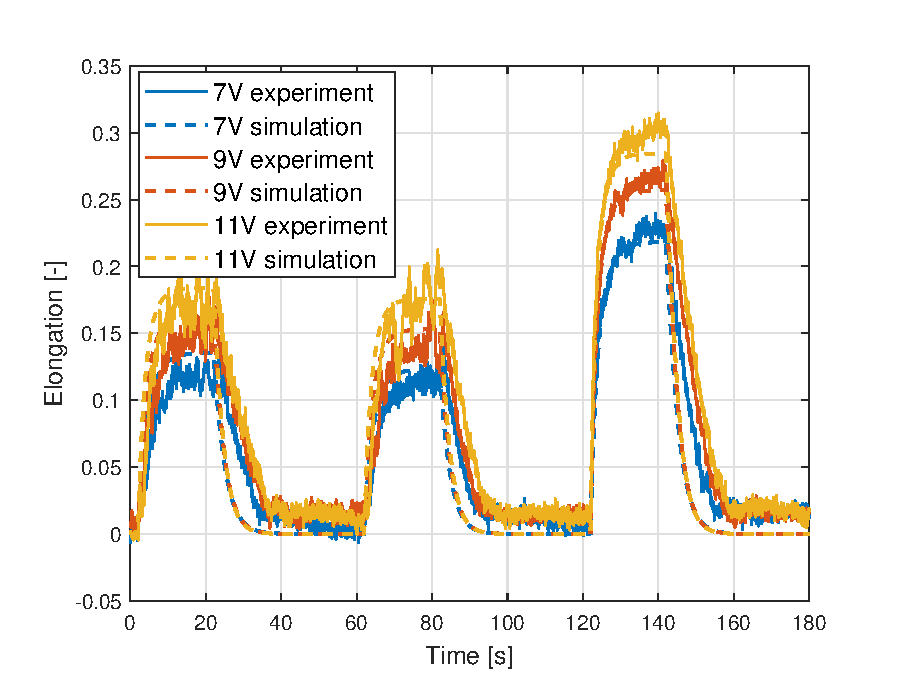
\includegraphics[width=\linewidth]{Figures/Chapter5/epsilonstiffnessver.eps} 
    \caption{Elongation for experiments (solid) and model (dotted) with scaled stiffness $K_\epsilon$. } 
    \label{fig5:elong} 
       \end{minipage} 
    \begin{minipage}[b]{0.49\linewidth}
     \centering
    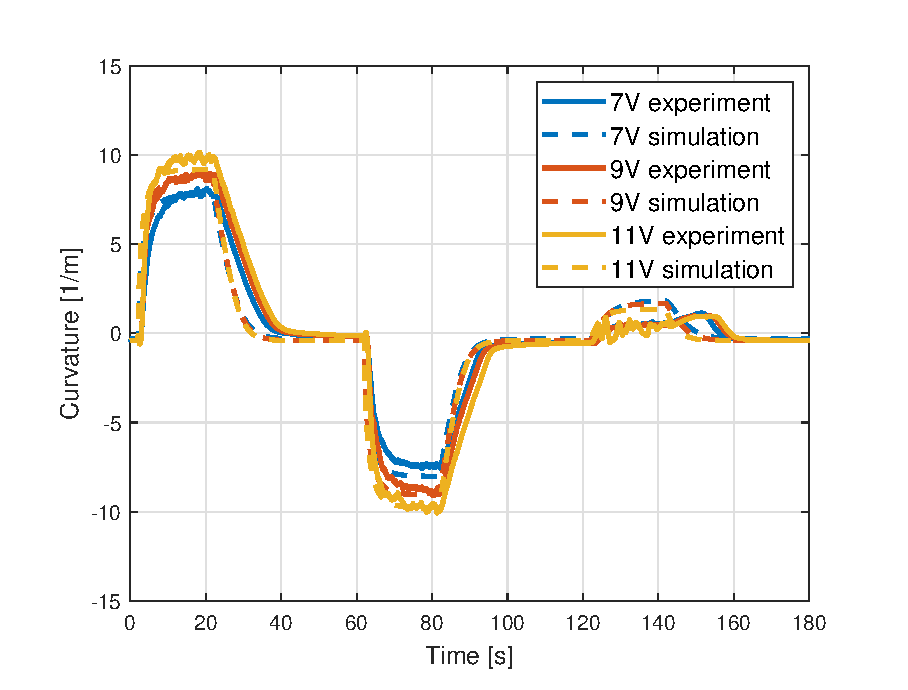
\includegraphics[width=\linewidth]{Figures/Chapter5/curvaturestiffnessver.eps}
    \caption{Curvature for experiments (solid) and model (dotted) with scaled stiffness $K_\kappa$. } 
    \label{fig5:kappa} 
    \end{minipage} 
\end{figure}

\begin{figure}[H] 
    \begin{minipage}[b]{0.49\linewidth}
     \centering
    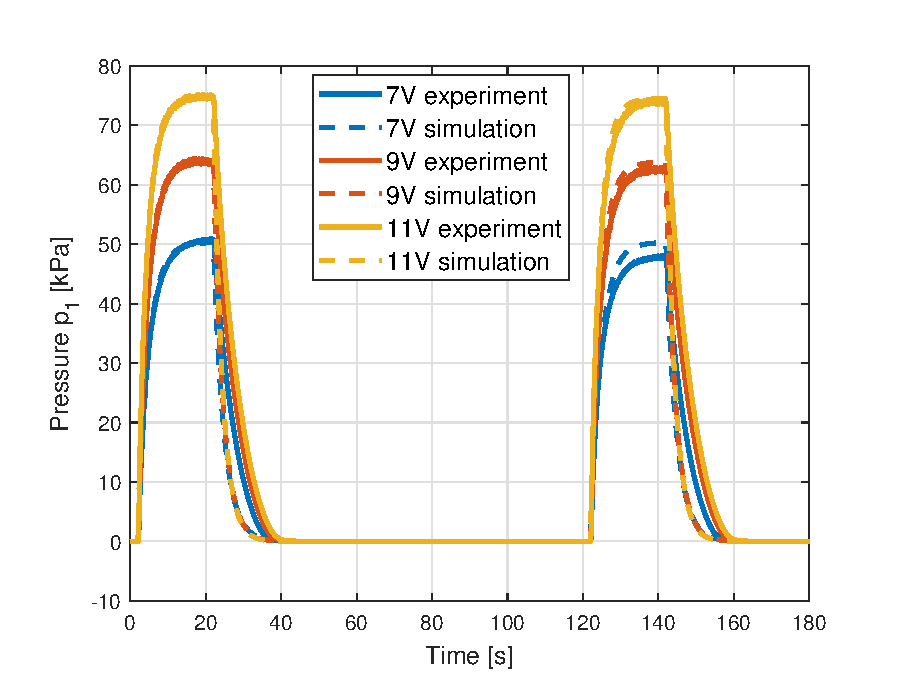
\includegraphics[width=\linewidth]{Figures/Chapter5/p1verif.eps} 
    \caption{Experimental and simulated bellow pressure $p_1$. } 
    \label{fig5:p1} 
       \end{minipage} 
    \begin{minipage}[b]{0.49\linewidth}
     \centering
    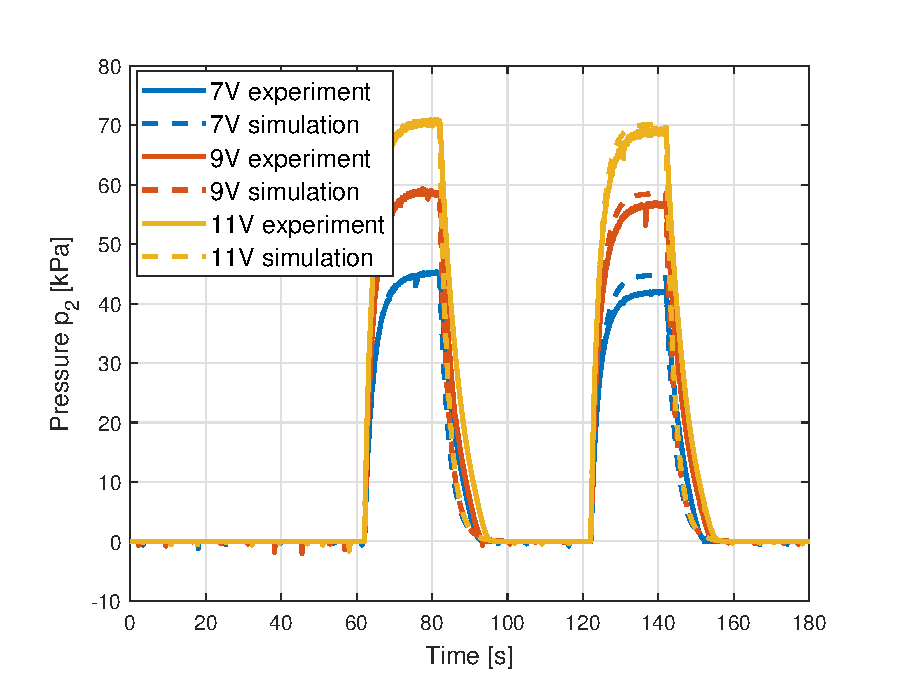
\includegraphics[width=\linewidth]{Figures/Chapter5/p2verif.eps} 
    \caption{Experimental and simulated bellow pressure $p_2$. } 
    \label{fig5:p2} 
    \end{minipage} 
\end{figure}




\subsection{Controller testing in simulation}

The controller is tested in simulation and experimentally. First, the controller will be tested on the developed dynamic model of the soft robot. The closed-loop response of the system to a step input is analyzed. This step input is also used for controller tuning. Subsequently, a reference signal is proposed to evaluate the tracking performance of the controller in simulation. 


\subsection*{Closed-loop step response in simulation}

A closed-loop step response with set-point $r_{set} = [-0.014,0.082]m$ is considered to verify the controller in simulation. This set-point demands the soft robot to bend and elongate, which allows tuning all gains of the Jacobian controller. First, the tuning of the Jacobian controller and pressure controller is provided. Then, the results of the step-response are presented and discussed. 

The controller in simulation is tuned according to the following procedure. First, the pressure controller gains $K_{pp}$ and $K_{ip}$ are set to $\text{diag}([1,1])$. Then, the proportional gains of the Jacobian controller $K_p$ are tuned. When tuning these parameters it is important that the Volt control input remains below the saturation limit. The gains $K_{p,1}$ and $K_{p,2}$ show an order of magnitude difference, as can be seen in Table \ref{tab5:gainssim}. This is caused by the input mapping as presented in Chapter \ref{chap3}. The moment and force mapping deviate approximately a factor of 100. Since the inverse mapping is used to set the reference pressure, large $K_{p,1}$ gains result in erroneous pressure set-points. Then the integrator gains $K_i$ are tuned. Relative high integration gains are necessary to accelerate error reduction. Lastly, the low-pass filter of the model-based controller is tuned. This gain is tuned such that it suppresses the system's eigenfrequencies. This frequency is excited by the control input dictated by the proportional gains at the beginning of the simulation. 



\begin{table}[H]
    \centering
     \caption{Controller gains used for step input in simulation.}
    \begin{tabular}{|c|c|} \hline
     \textbf{Tuning Parameter}    & \textbf{Value}  \\ \hline
    $K_p$ & $\text{diag}([300,3000])$  \\ \hline
    $K_i$ & $\text{diag}([17500,17500])$  \\ \hline
    $K_{pp}$ & $\text{diag}([1,1])$  \\ \hline
    $K_{ip}$ & $\text{diag}([1,1])$ \\ \hline
    $\zeta$ & 0.01 \\ \hline
    \end{tabular}

    \label{tab5:gainssim}
\end{table}

The results of the step response in the simulation are presented in Figures \ref{fig5:errorsim} to \ref{fig5:pressuresim}. The error response as a function of time is displayed in Figure \ref{fig5:errorsim}. It can be seen that the initial error in x and y-direction is 14 and 12 mm, respectively. For both errors, it takes about 16 seconds to reach 0 steady-state error. In the first 0.4 seconds, an almost linear error decrease is observed, caused by the proportional gains. Then, the error response shows first-order system behaviour. This is caused by the pump dynamics which act as low pass filters. Additionally, the low-pass filter of the model-based controller filters high frequent oscillations. Both factors result in smooth yet slow error convergence. Due to the low-pass filter, oscillations in the error signal are largely reduced. The observed eigenfrequencies for bending and elongation are 40 and 130 Hz, respectively. This indicates that the stiffness to mass ratio is higher than expected. Since the stiffness has been experimentally determined, the mass approximation causes these high eigenfrequencies.



\begin{figure}[H]
    \centering
\begin{minipage}{0.5\textwidth}
        \centering
        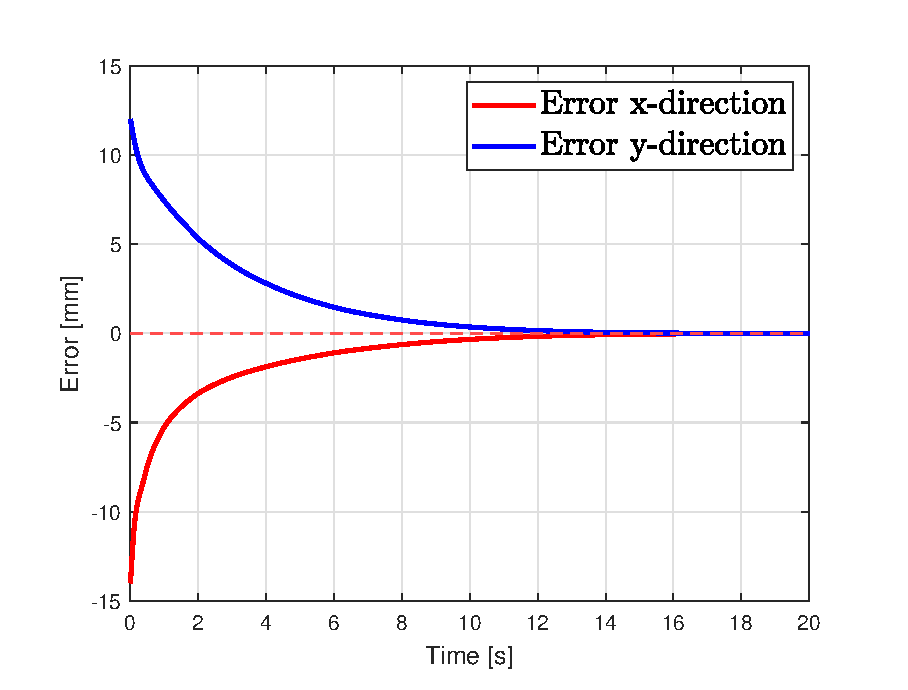
\includegraphics[width=\textwidth]{Figures/Chapter5/stepsimerror.eps} 
        \caption{Error in x and y-direction as a function of time.}
        \label{fig5:errorsim}
    \end{minipage}\hfill
    \begin{minipage}{0.5\textwidth}
        \centering
        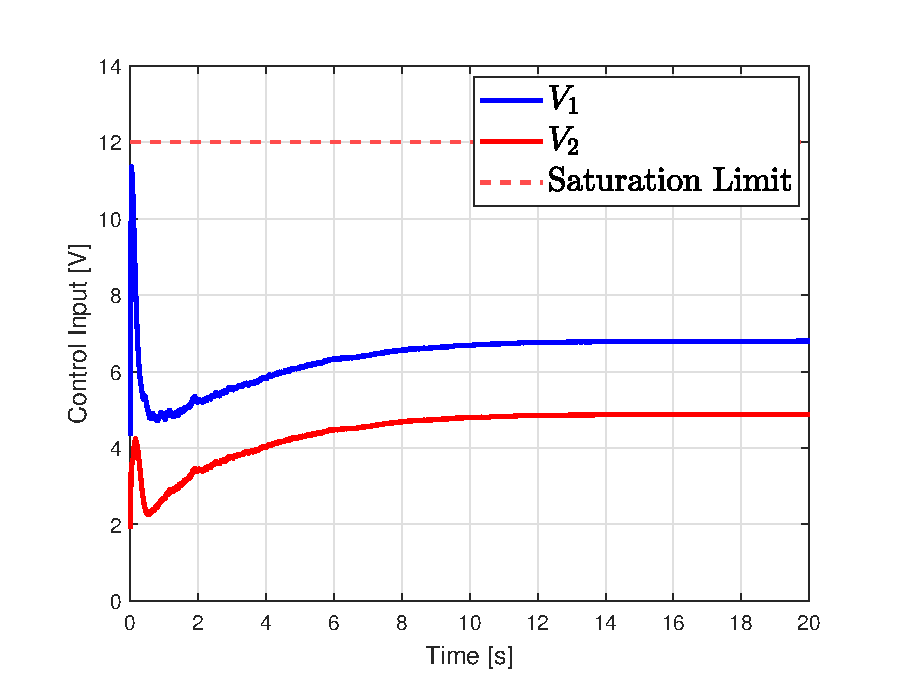
\includegraphics[width=\textwidth]{Figures/Chapter5/stepsiminputV.eps} 
        \caption{Control input to the air pumps as a function of time}
        \label{fig5:controlinputsim}
    \end{minipage}
\end{figure}


\begin{figure}[H]
\centering
\begin{minipage}{0.5\textwidth}
        \centering
        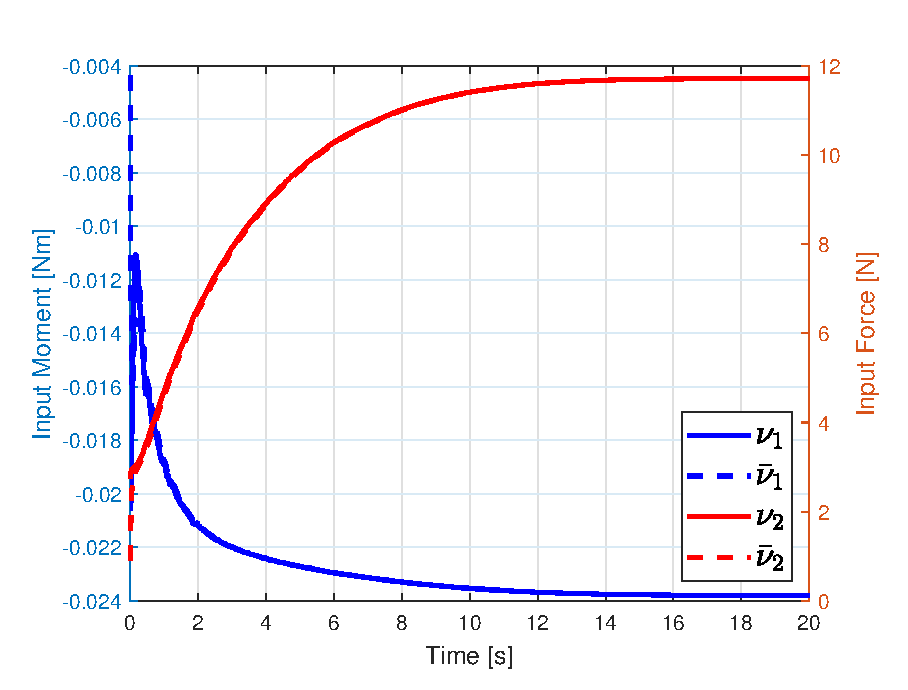
\includegraphics[width=\textwidth]{Figures/Chapter5/jacinputstepsim.eps} 
        \caption{Input moment and force as determined by Jacobian controller. Solid line is unfiltered, dotted line is low-pass filtered}
        \label{fig5:inputsim}

    \end{minipage}\hfill
    \begin{minipage}{0.5\textwidth}
        \centering
        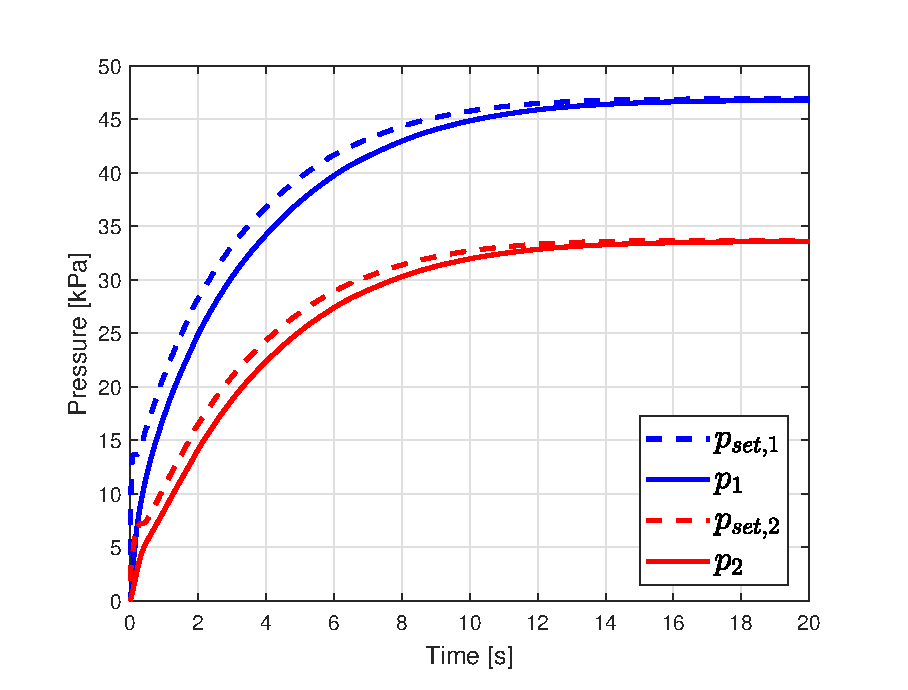
\includegraphics[width=\textwidth]{Figures/Chapter5/pressuresimstep.eps}
        \caption{Pressure response, dotted lines indicate reference pressure, solid lines are simulated pressures.}
        \label{fig5:pressuresim}
    \end{minipage}
\end{figure}




Figure \ref{fig5:controlinputsim} shows the control input to the pump model. During the first seconds, the effects of high proportional gains can be observed. Initiated by a large initial error, the input to the air pumps show a peak during the first 0.3 seconds. This causes the error to rapidly decrease, especially in the x-direction. In reaction to this, the proportional gain decreases its control effort, resulting in a dip observed at 0.5 seconds. From then on the integrator is mostly responsible for the error decrease, as the control input to the air pumps slowly increases. Eventually, the input to the air pumps is around 6.7 and 4.8 Volt. 

Figure \ref{fig5:inputsim} displays the input moment and force as determined by the model-based controller. The dotted lines show the low-pass filtered input which is the input to the air pumps. It can be seen that although $\zeta$ is chosen just 0.01 [-], the delay is small over the complete 20 second time window. The low-pass filter has a major influence during the first few seconds. In this region, it attenuates high-frequency control input changes which are caused by the excited system dynamics. 


Lastly, Figure \ref{fig5:pressuresim} shows the pressure response in simulation. The dotted lines indicate reference pressure, and the solid lines mark the simulated attained pressure. The figure shows that after 16 seconds a constant bellow pressure is obtained. This coincides with the position error being zero after this time.



\subsection*{Closed-loop reference tracking in simulation}

Now the controller has been tested and tuned for a step response, its performance is analyzed for a reference tracking problem. The reference tracking problem that is being considered is similar to the ellipsoid reference path of \cite{berkers}. Therefore, the outcomes of this work can be well compared to the latter work. The ellipsoid reference path is described by the following equations,

\begin{equation}
    x_{ref} = \begin{cases} 
      0 &  0 \leq t < t_1 \\
     a \sin(2\pi \frac{t - t_1}{T_{ell}}) &t_1 \leq t  < T_{ell} + t_1 \\
     0 & t \geq T_{ell} + t_1
   \end{cases} 
\end{equation}

and,


\begin{equation}
    y_{ref} = \begin{cases} 
       y_{off} &  0 \leq t < t_1 \\
     (y_{off} +b) -  b \cos(2\pi \frac{t - t_1}{T_{ell}}) & t_1 \leq t < T_{ell} + t_1 \\
     y_{off} & t \geq T_{ell} + t_1
   \end{cases}  
   \end{equation}

where it can be seen that during the first $t_1$ seconds the reference position is equal to offset $y_{off}$. Then, a clockwise rotation occurs during $T_{ell}$ seconds in which the amplitude in the x-direction is $a$, and the maximum elongation in y-direction is $y_{off} + 2b$. After one period the reference signal remains equal to its offset position. The values of these parameters are shown in Table \ref{tab5:refparamssim}. Since the controller has no feedforward control and considering the slow dynamics of the system, $T_{ell}$ is chosen 400 seconds. The amplitudes, $a$ and $b$ are comparable to the step inputs.


\begin{table}[H]
    \centering
    \caption{Reference tracking parameters in simulation}
    \begin{tabular}{|c|c|} \hline
   \textbf{Parameter}  & \textbf{Value [unit]} \\ \hline
    $t_1$ &   15 [s]  \\ 
    $y_{off}$ & 0.074 [mm] \\
    $a$ & 13 [mm] \\
    $b$ & 7 [mm] \\
    $T_{ell}$ & 400 [s] \\ \hline
\end{tabular}
    \label{tab5:refparamssim}
\end{table}


The results of this ellipsoid reference in the x-y plane are shown in Figure \ref{fig5:xysim}. In this figure, the green crosses indicate the reference position at a given time. The red crosses mark the actual position at this time instant. A delay is observed between the reference and actual position, which is to be expected for a feedback controller. However, this delay is not constant during tracking. The measured delay between the reference position and actual position at 200 seconds is about 3.2 seconds, while a delay of only 1.3 seconds is observed at 400 seconds. The cause of this behaviour is related to the pump dynamics, as for larger reference pressures the delay increases. Overall, the controller is able to track the reference trajectory fairly accurate. Taking into account an average delay of 2.12 seconds, the root mean square (RMS) errors while tracking the ellipsoid reference path are $e_{x,RMS} = 0.1489 \hspace{2pt} mm$ and $e_{y,RMS} =0.0899 \hspace{2pt} mm$ in x and y-direction, respectively.

\begin{figure}[H] 
    \begin{minipage}[b]{0.49\linewidth}
     \centering
    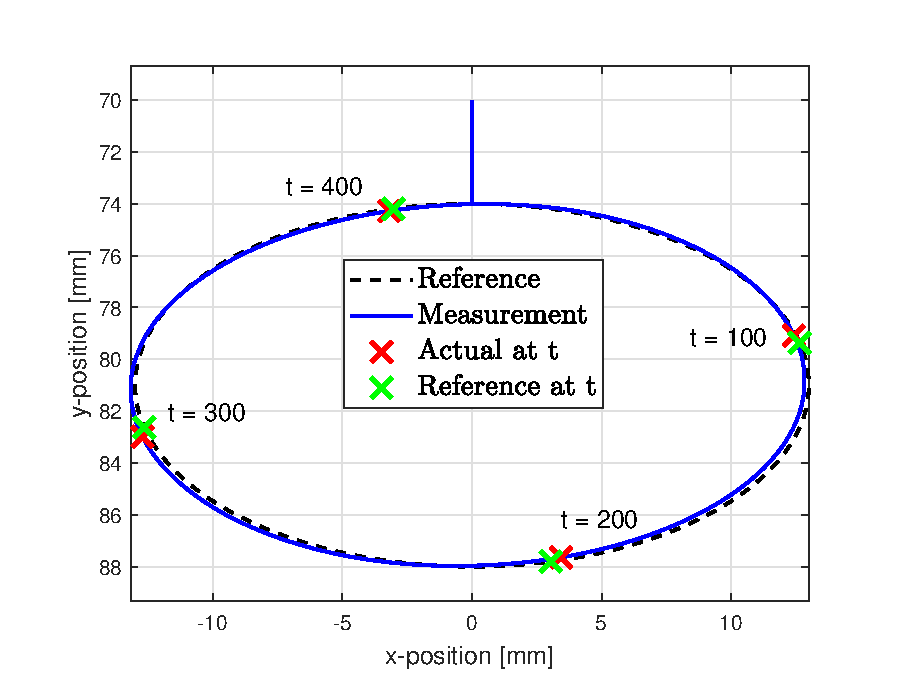
\includegraphics[width=\linewidth]{Figures/Chapter5/ellipssim.eps} 
    \caption{Position in the x,y-plane for the ellipsoid reference path.} 
    \label{fig5:xysim} 
       \end{minipage} 
    \begin{minipage}[b]{0.49\linewidth}
     \centering
    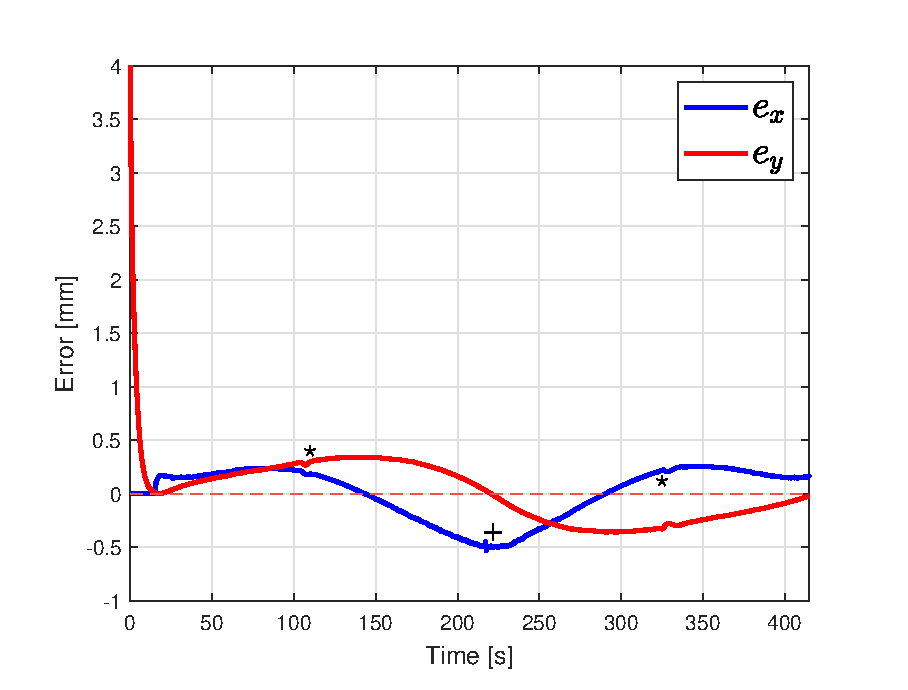
\includegraphics[width=\linewidth]{Figures/Chapter5/errorellipssim.eps} 
    \caption{Error in the x and y-direction as a function of time for an ellipsoid reference path.} 
    \label{fig5:errorxyellipssim} 
    \end{minipage} 
\end{figure}


The error profiles are shown in Figure \ref{fig5:errorxyellipssim}. The first 15 seconds show a relatively large error in the y-direction as the soft robot is elongating to its offset position. The error that follows shows a sinusoidal shape, as is expected for a sinusoidal reference signal. This kind of error profile can be resolved by feedforward control. The error response shows two characteristics with respect to angle changes. At 107 seconds and 327 seconds, the error response shows a disturbance in both error signals, indicated by a `$*$'. This is caused by a change in curvature rate. For the first instant, the angular rate changes from positive to negative. At the second instance, the exact opposite occurs, here the negative angular rate changes to a positive angular rate. This rate change affects the Jacobian causing a disturbance on position level. At 217 seconds a similar disturbance can be observed, denoted by a `$+$'. Again this is related to the curvature. At this time instant the curvature changes sign, again affecting the Jacobian and thus position. It should be noted that this disturbance is only present in $e_x$.




Figure \ref{fig5:controlinputellipssim} shows the control input determined by the model-based controller, pressure response and control input to the simulated air pumps, respectively. The top figure shows a sinusoidal reference moment. Its extrema are situated at the times the x-displacement is largest. Likewise, the force input reaches a maximum when the maximum y-displacement is required. This coincides with the observations in the pressure response shown in the centre figure. Note that on this time scale the average 2.12 second delay between reference moment and force and pressure can not be distinguished. The bottom figure shows the control input to the air pumps.



\begin{figure}[H]
    \centering
    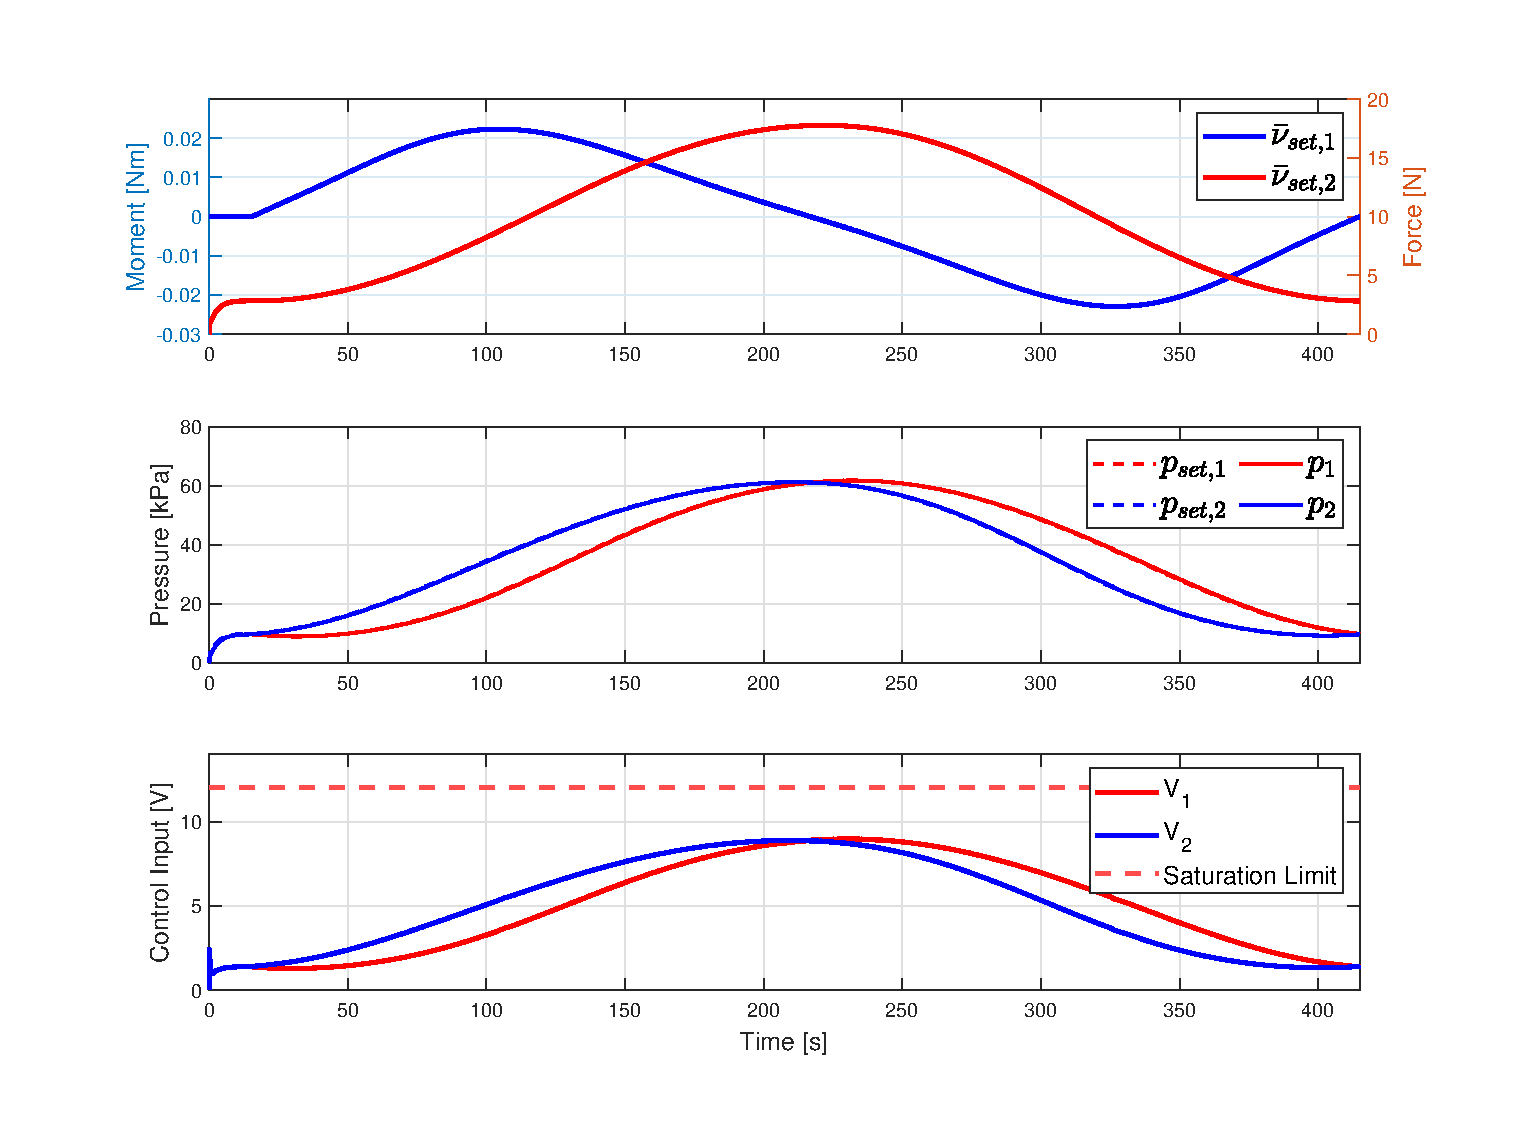
\includegraphics[width = \textwidth]{Figures/Chapter5/controlinputsimell.eps}
    \caption{\textbf{Top:} Input moment and force determined by model-based controller. \textbf{Middle:} Bellow pressure during ellipsoid reference tracking. \textbf{Bottom:} Control input to the air pumps in simulation.}
    \label{fig5:controlinputellipssim}
\end{figure}



\subsection{Controller testing in experiments}

Now the controller is implemented in simulation, the experimental case is considered. Therefore, the experimental setup is first detailed. Also, the digital filter design and revision of the input mapping are explained. Then, the controller is tuned for a step response in experiments. To verify if the manipulator has symmetrical stiffness properties, bending in both bending directions is analyzed. Finally, the reference tracking problem in experiments is presented. 


\subsection*{Experimental setup}

\begin{figure}[H]
    \centering
    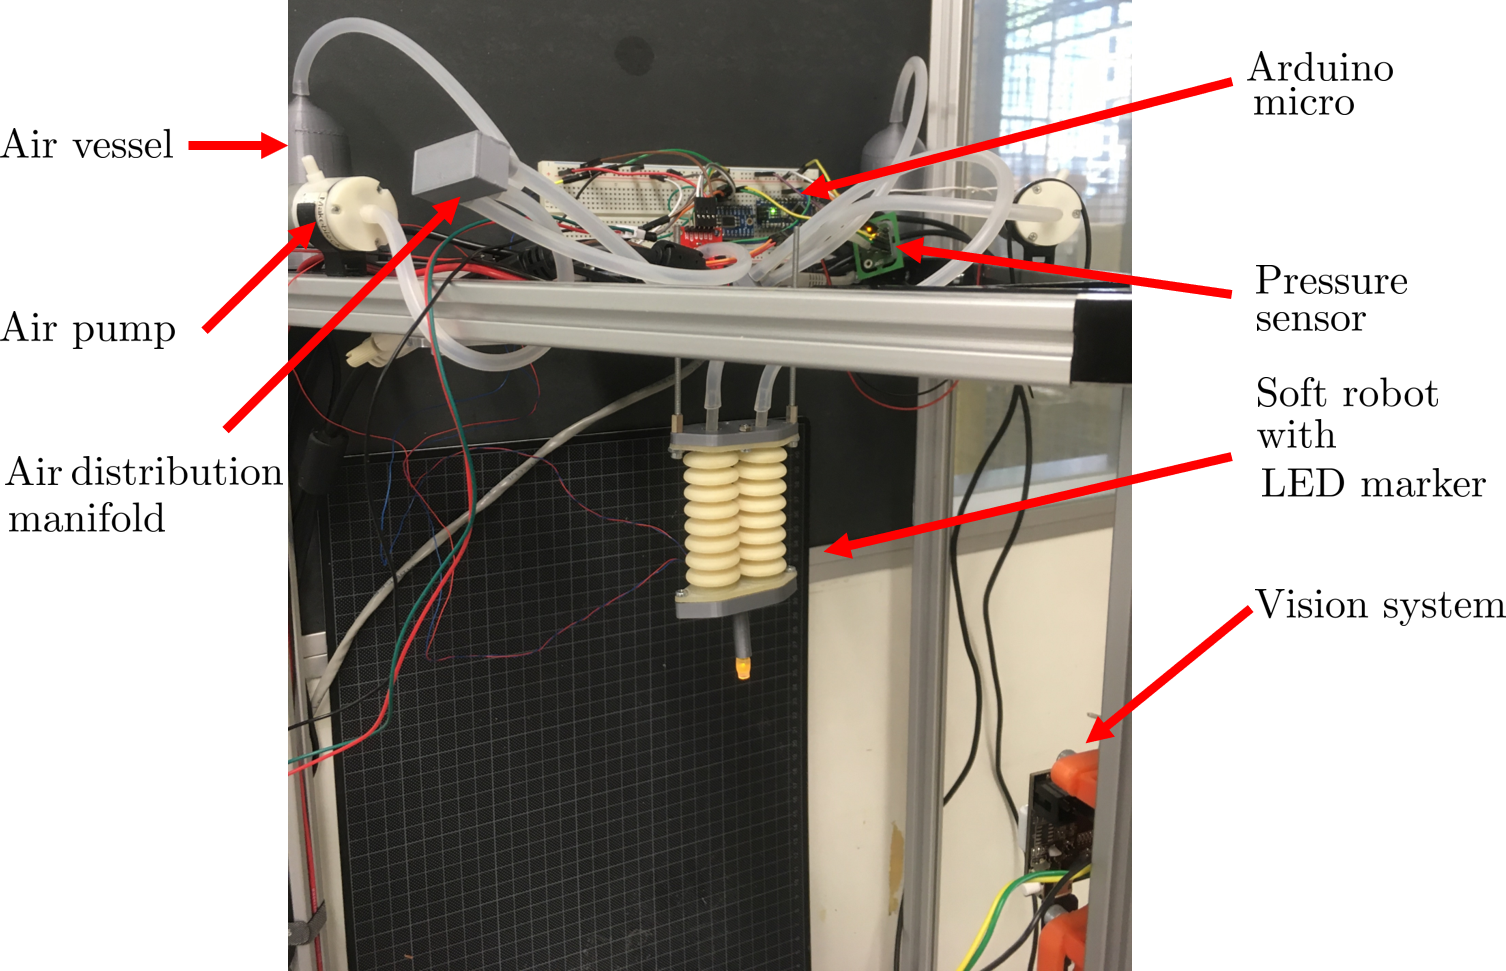
\includegraphics[width = \textwidth]{Figures/Chapter5/expsetup.png}
    \caption{Experimental setup of the soft robot.}
    \label{fig5:setup}
\end{figure}

Figure \ref{fig5:setup} shows the experimental soft robot setup as is present in the laboratory. The soft robot in the centre of the figure is mounted to the top of its supportive structure by threaded rods. To the soft robot itself, an LED and IMU carrier are connected. Furthermore, the two air inlets at the top of the soft robot can be seen. Each of these air inlets is in contact with an air pump as follows. Each air pump is attached to an air distribution manifold via a hose. This distribution manifold has three air outlets. To these outlets, a pressure sensor, air tank and actuator bellow are attached, respectively. To this end, silicone hoses with an inner diameter of 3 millimetres are used. To the tip of the actuator, a yellow LED is mounted that is used for optical tracking. This LED is glued to a connector that has been additively manufactured. The LED has an offset of 35 millimetres with respect to the tip of the actuator. This connector part also houses the IMU. This IMU is used to measure the rotation of the actuator's tip. Furthermore, a vision system is focused on the actuator. This vision system is programmed such that it can recognise and track the LED marker. The actual end-effector position can then be calculated utilizing trigonometry using rotation and position data, see Appendix \ref{app:chap5} for this derivation.



The sensors described above, e.g. the IMU, two pressure sensors and optical tracking system are connected to an Arduino micro. The Arduino acts as an intermediate sensor processor that buffers the data and compactly transmits them to the Raspberry PI via Serial Communication. The maximum attained sampling frequency of the Arduino is 40 Hz. On the Raspberry, the model-based controller and pressure controller are programmed. To the Raspberry, an ADC converter shield is mounted which can regulate the Volt input to the air pumps. The Raspberry PI can receive sensor data and perform all necessary calculations at a frequency of 25 Hz. This is the maximum bandwidth frequency of the control system. Considering the slow system dynamics in the order of 1 Hz \cite{tawk2018bioinspired},\cite{HighBandwidthControl} this sampling frequency well suffices.





\subsection*{Digital filter design}

Since sensory devices are prone to measurement noise and disturbances, digital filters are implemented. For the IMU two different filters are applied. For the pressure and visions system, a single filter is used. 

For the IMU two filters are used to decrease noise and disturbances. First, the angle is filtered by a complementary filter, then a moving average filter is applied. The IMU houses an accelerometer, gyroscope and temperature sensor. The first two are necessary to determine rotation. The accelerometer measures acceleration based on force, whereas the gyroscope allows for the measurement of rotational velocity. The output of both sensors is utilized to calculate rotation. The accelerometer and gyroscope each have their deficits. The accelerometer exploits force measurements to determine acceleration. This also includes actuation forces, hence undesired high frequent pump dynamics influence the accelerometer readings. The gyroscope, on the other side, is prone to drift which becomes a problem over time. A complementary filter can be used to enhance angle calculations as this filter fuses gyroscopic data with acceleration data. To remove high-frequency noise the acceleration data is low-pass filtered, whereas gyroscope data is high-pass filtered. Therefore, the complementary filter can be described as, 

\begin{equation}
    \theta = \delta \theta_{acc} + (1-\delta) \int_0^t \omega_{gyr} \hspace{2pt} ds    \hspace{25pt} \text{with}  \hspace{10pt} \theta_{acc} = \atantwo(a_y,a_x)
\end{equation}

where $\theta_{acc}$ is the calculated angle based on the measured accelerations $a_y$ and $a_x$ in the IMU's y-direction and x-direction, respectively. The angular velocity $\omega_{gyr}$ is measured by the IMU's gyroscope. Parameter $0 < \delta \leq 1$ determines the relative importance between acceleration and gyroscope data. Since the angle readings with a complementary filter are not deemed satisfactory, an additional moving average filter is implemented. Solely using the complementary filter showed high amplitude oscillatory angle changes, whilst the tip velocity was near zero. The moving average filter reduces the amplitude of these oscillations as past angle data is used in the updated angle reading. The moving average filter is given as,

\begin{equation}
    \Bar{\theta}_k = \frac{1}{N_{IMU}}\sum_{i = 0} ^ {N_{IMU}-1} \theta_{k-i}
\end{equation}

where $\Bar{\theta}_k$ is the averaged output, $N_{IMU}$ the number of past samples to average and $\theta_{k-i}$ the past angle sample. It must be noted that both filters cause delays in the system. Therefore the tuning should be done carefully, as stability is not guaranteed.

The vision system which tracks the LED marker gives out its position data in pixels. These pixels are integer numbers, causing discrete steps in the position measurement. To remove these steps and represent the mean position during a sampling instant, the data is low-pass filtered. The description of the low-pass filter is identical to (\ref{eq4:lowpass}) and given as,

\begin{equation}
\bar{r}_{pixy,k} = \zeta_{pixy} r_{pixy,k} + (1-\zeta_{pixy})\bar{r}_{pixy,k-1}
\label{eq5:lowpass}
\end{equation}

where $\Bar{r}_{pixy,k}$ is the low-pass filtered position vector of the LED marker given in pixels. The sampled position vector is $r_{pixy,k}$ and $\bar{r}_{pixy,k-1}$ the previous filtered position. Parameter $\zeta$ determines the cut-off frequency of the low-pass filter. High values for $\zeta$ prioritize recent samples, whereas low values stress past LED positions. The pressure data is also low-pass filtered, following an identical procedure as the position data. For this variable, the weighing is indicated by $\zeta_p$. 





\subsection*{Revision of input mapping}

The accuracy of the obtained input mapping in Chapter \ref{chap3} as given by (\ref{eq3:H}) was questioned during the experiments. Recall that this mapping is employed to map moment and force to individual bellow pressure. Since the entries in the mapping matrix deviated an order of magnitude of 2, tuning the controller gains is cumbersome. When using equivalent order of gains in the model-based controller, the reference pressure for both bellows is almost identical. This makes tuning of the curvature gain $K_{p,1}$ hard. To overcome this problem the input mapping is revised as follows. 

First, the pressure controller gains are set as $K_{pp} =\text{diag}([1,1])$ and the integrator gain $K_{ip} = \text{diag}([0,0])$. In this way, the actual system pressure will never converge to the reference pressure. Subsequently, a setpoint is chosen for which the soft robot needs to elongate and bend. The proportional gain and integration gain of the Jacobian controller are chosen such that the steady-state is reached within a reasonable time. Eventually, the soft robot will move to its desired position setpoint, as the integrator action in the model-based controller will increase $\bar{\nu}_{set}$. Once the reference position is reached, the input signal $\bar{\nu}_{set}$ as determined with the old mapping remains constant. Furthermore, the actual system pressure in both bellows is known. Based on the pressures, and value of $\bar{\nu}_{set}$ the entries of the input mapping can be redetermined. Following this procedure, the revised input mapping was found as,

\begin{equation}
    H = \begin{bmatrix} 	0.0206 &  -0.0206 \\ 
	0.1808 & 0.1808 \end{bmatrix},
    \label{eq4:revisedH}
\end{equation}

where it can be seen that the moment to pressure mapping has increased by a factor of 10. The force mapping is found of equal order of magnitude. A disadvantage of this method is that the newly obtained mapping matrix still depends on the initial mapping. Evidently, the $\bar{\nu}_{set}$ is obtained with the old mapping. Therefore this mapping should be regarded as some sort of tuning mapping, defining the relative importance between force and moment. Hereto, the physical interpretation of reference force in Newton and moment in Newton-meter is lost to some extend. 

\subsection*{Experimental tuning procedure}

Since the model deviates from the actual system, the controllers need to be tuned for the experimental setup. The used parameters are found by iterative tuning and observing the system's response for the step input $r_{set} = [-0.014,0.082]m$. 

The tuning of the system is done according to the following procedure. Initially, the proportional gains $K_{pp}$ of the pressure controller are set as $\text{diag}([1,1])$. The integrator gains $K_{ip}$ are left as $\text{diag([0,0])}$. Subsequently, the low-pass filter gains on the sensors $\zeta_p$, $\zeta_{pixy}$ are set relatively high ($>0.9$), to minimize delays. Likewise, the sample amount of the moving average filter $N_{IMU}$ can be chosen low ($<5$). The complementary filter $\delta_{IMU}$ is taken initially as 0.02 \cite{compfilter}. These values allow passing through almost all recent data with a relatively small delay. Then the set-point $r_{set} = [0.014,0.082]^\top$ is selected. The proportional gains of the Jacobian controller $K_p$ are increased, such that the system does not saturate in the first few seconds of its response. Recall that the first entry $K_{p,1}$ affects the moment, and $K_{p,2}$ affect the force reference. Increasing the value of $K_{p,1}$ will result in a swing-like motion in the first seconds, caused by the initially large error in the x-direction. To minimize this behaviour, gain $K_{p,1}$ should be chosen smaller than $K_{p,2}$. At this point, the integrator gain of the pressure controller $K_{ip}$ can be increased to allow tracking of the pressure setpoint. Furthermore, the integrator gains $K_i$ can be tuned, these should be chosen relatively high to speed up error attenuation. The integrator gains are chosen too high when overshoot is observed. Since the system can not be actively deflated, and deflation rates are low, the integrator is not able to compensate well for overshoot. Next, the low-pass filter of the Jacobian controller $\zeta$ can be tuned. This parameter should be decreased to obtain a smooth input signal. At this point $\zeta_{pixy}$ can be tuned as well, to obtain a smoother position signal. Once the control input is smooth, the pressure response is considered. This response can be smoothed by decreasing the low-pass gain $\zeta_p$. Lastly, the sample amount $N_{IMU}$ of the moving average filter is tuned. Once this procedure is completed, the system can be further fine-tuned to increase performance. Table \ref{tab5:tuningcosiderations} shows some guidelines and considerations whilst tuning the controller.



\begin{table}[H]
    \centering
     \caption{Tuning considerations experimental tuning.}
    % \scalebox{0.95}{
\begin{tabular}{p{2.5cm} p{9cm} p{3cm}} \hline
%    \begin{tabular}{p{2cm} p{11cm} p{2.5cm}} \hline
      \textbf{Parameter}   & \textbf{Tuning  consideration} & \textbf{Value } \\ \hline
      $K_p$   &   $K_{p,1}$ affects curvature, whereas $K_{p,2}$ influences elongation. To decrease a swing like motion $K_{p,1} < K_{p,2}$. Motor saturation should be considered whilst tuning.   &  diag([$1750,3750$])            \\ \hline
      $K_i$   &   $K_{i,1}$ acts on the moment, to compensate for lower gain, this parameter can be increased. When the gains $K_p$ are set, $K_i$ can be increased up until error overshoot occurs.   &  diag([$6500,6250$])    \\ \hline
      $K_{pp}$   &  Is a scalar matrix due to assumed equal pump characters. It is not recommended to chose $K_{pp} >1$ as this results in poor performance. Smaller values will result in a smoother Volt input at the cost of performance.  &  diag([$1 ,1$])     \\ \hline
      $K_{ip}$   &  The integrator gains should be chosen such that system pressure tracks the reference pressure signal. If chosen too high, the system saturates the first seconds if used with high model-based control gains.    &  diag([$0.75,0.75$])    \\ \hline
      $\zeta$    &   This parameter allows to create smooth reference control input. A weigh-off is made between smoothness and delay. &  $0.08$  \\ \hline
      $\zeta_p$    &   This parameter majorly influences the control input. A smooth pressure reading will result in a smoother control input $V$. Too low values will result in stability problems.   & $0.25$ $[-]$  \\ \hline
      $\zeta_{pixy}$    &  Since the vision system uses discretized pixel coordinates, a filter can be used to estimate position during a sample instant. Delays should be considered and minimized     & $0.25$   \\ \hline
      $N_{IMU}$    &  This value should be tuned such that large oscillations in the angle readings are minimized, whilst reducing the delay as much as possible. & $35$   \\ \hline
      $\delta_{IMU}$    &  High values stress importance of accelerometer readings, low values emphasize gyroscopic data. Since the actuator forces affect accelerometer readings it is recommended not to chose $\delta_{IMU}$ too high.  & $0.08$  \\ \hline
    \end{tabular}
    \label{tab5:tuningcosiderations}
\end{table}


\subsection*{Closed-loop step response in experiments}


The performance of the designed controller is assessed by analyzing the system's step response in experiments. For the experimental testing, two set-points are considered. As for the simulation, the first set-point is similar to $r_{set} = [-0.014,0.082] m$. The second set-point is mirrored and described by $r_{set} = [0.014,0.082] m$. These set-points enable analyzing the movement in both Cartesian directions. Since it is assumed that the soft robot is perfectly symmetric and the air pumps have equal characteristics, it is expected that the system's response will be similar.

The system's error response as a function of time to set-point $r_{set} = [-0.014,0.082] m$ is given in Figure \ref{fig5:errorswingleft}. The figure shows the error signal in both directions. In the physical setup, this set-point corresponds to a tip-movement to the left, hence ``left"  is used to address this set-point. A video is provided by clicking the link in the caption. The Volt input to the air pumps is presented in Figure \ref{fig5:inputswingleft}. Furthermore, Figure \ref{fig5:nuleft} shows control input $\bar{\nu}_{set}$ as determined by the model-based controller. This figure also shows the unfiltered control input $\nu$. Figure \ref{fig5:pleft} shows the bellow pressure of both bellows as solid lines. The dotted lines in this figure indicate the reference pressure.

Figure \ref{fig5:errorswingleft} shows an initial error of 14 $mm$ and 12 $mm$ in the x and y-direction, respectively. Both initial errors correspond to the desired set-point. As the initial error is largest, the proportional gain responds by increasing the Volt input, as can be seen in Figure \ref{fig5:inputswingleft}. This results in a rapid decrease in error, causing a swing-like motion between 0.5 and 1.5 seconds. After 1.5 seconds, the integrator takes over and the speed at which the error decreases slows down. After 12 seconds the steady-state is reached for the x-direction, which coincides with a steady-state input moment of -0.6$Nm$, as shown in Figure \ref{fig5:nuleft}. For the y-direction the steady-state is reached after 8 seconds, coinciding with a steady-state input force of 13 $N$. 


\begin{figure}[H] 
    \begin{minipage}[b]{0.49\linewidth}
     \centering
    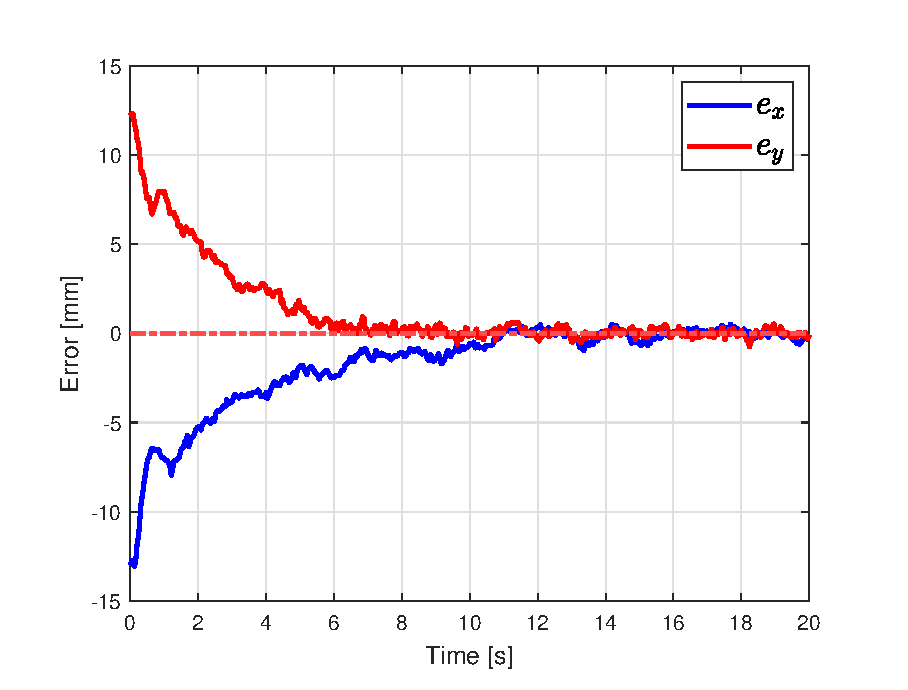
\includegraphics[width=\linewidth]{Figures/Chapter5/errrorstepleft.eps} 
    \caption{Error response in x and y-direction.Video provided at URL: \url{https://youtu.be/xz6EJKAM77Q}} 
    \label{fig5:errorswingleft} 
       \end{minipage} 
    \begin{minipage}[b]{0.49\linewidth}
     \centering
    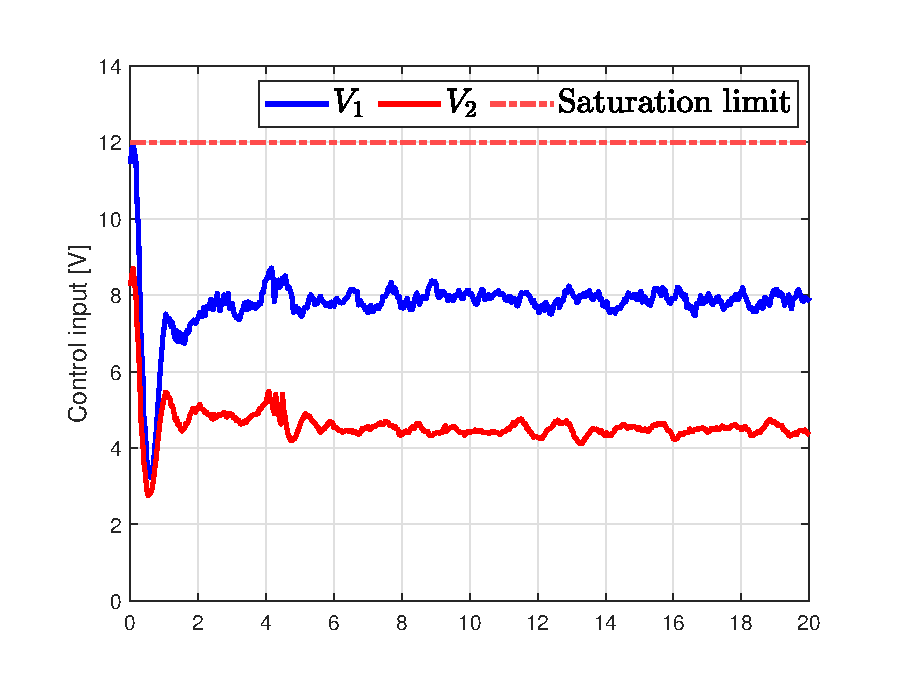
\includegraphics[width=\linewidth]{Figures/Chapter5/controlinputstepleftV.eps} 
    \caption{Volt control input signal to the air pumps.} 
    \vspace{12pt}
    \label{fig5:inputswingleft} 
    \end{minipage} 
\end{figure}

\clearpage


\begin{figure}[H] 
    \begin{minipage}[b]{0.49\linewidth}
     \centering
    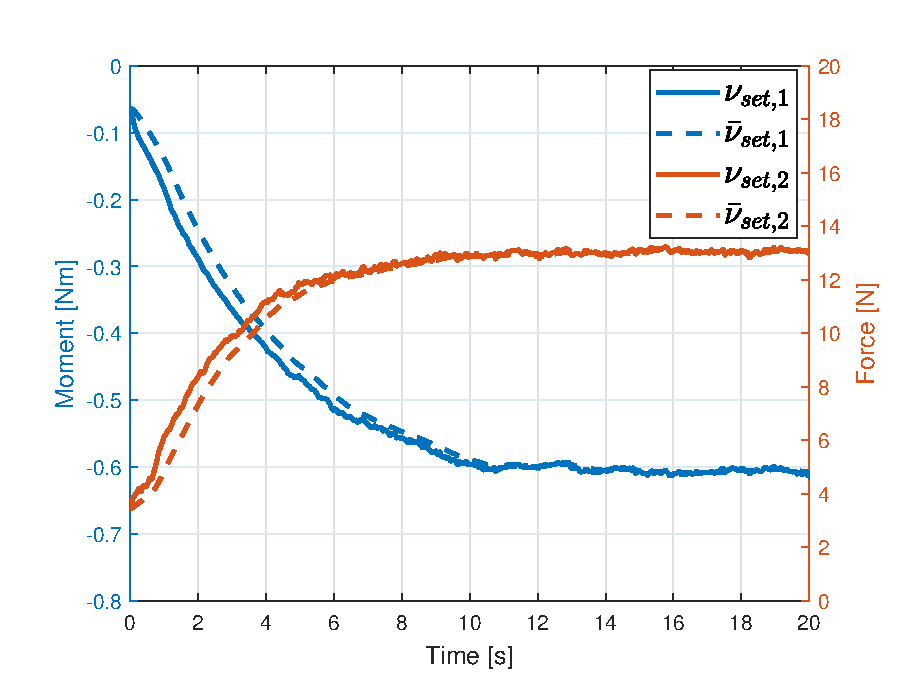
\includegraphics[width=\linewidth]{Figures/Chapter5/jacinputstepleft.eps} 
    \caption{Input moment and force as determined by Jacobian controller. Solid line is unfiltered input, dotted line low-pass filtered. } 
    \label{fig5:nuleft} 
       \end{minipage} 
    \begin{minipage}[b]{0.49\linewidth}
     \centering
    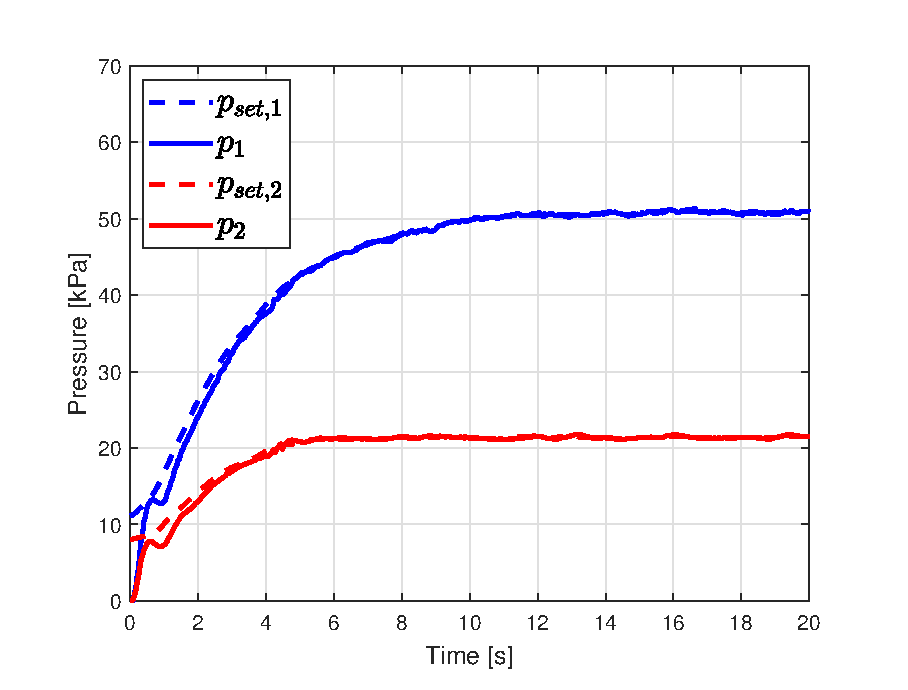
\includegraphics[width=\linewidth]{Figures/Chapter5/pressurestepleft.eps} 
    \caption{Pressure response, dotted lines indicate reference pressure, solid lines are measured pressures.} 
    \label{fig5:pleft} 
    \end{minipage} 
\end{figure}

The control input to the pumps is shown in Figure \ref{fig5:inputswingleft}. The first 1.5 seconds demonstrate the effect of the proportional gains. In this region, the initial error in both directions is largest. After around 10 seconds input $V_1$ and $V_2$ remain around the 5.3V and 8V, respectively. Figure \ref{fig5:pleft} shows the pressure in each bellow. It can be seen that the actual bellow pressure is tracking the pressure reference after 5 seconds and remains close to this reference for the continuation of the experiment. The eventual steady-state pressure $p_1$ is equal to 51 kPa, the measured pressure $p_2$ is 21.3 kPa. 


%%%%%%%%%%%%%%%


As mentioned, the first set-point is mirrored to check if the soft robot has equal characteristics when bending in the opposite direction. For this step response the setpoint is $r_{set} = [0.014,0.082]^\top$. This set-point is denoted as the ``right".


The error response in both Cartesian directions are shown in Figure \ref{fig5:errorswingright}. Compared to the left set-point, this right set-point does not clearly show a swing during the first 1.5 seconds. Instead, a more gradual error decrease is observed. In x-direction, the steady-state error is reached after about 14 seconds. At this time instant the input moment, as depicted in Figure \ref{fig5:nuright}, has a value of 0.78 $Nm$. For the left set-point, a steady-state input moment of -0.6 $Nm$ was observed. This indicates that the bending stiffness is not exactly symmetrical for both bending directions. This can also be concluded based on the pressure response. For the right set-point, a maximum steady-state pressure of 60 $kPa$ is measured, as can be seen in Figure \ref{fig5:pright}. The steady-state pressure for the left set-point is equal to 51 $kPa$. The error in y-direction for the right set-point shows similar behaviour as for the left set-point. The settling time is around 10 seconds and has a steady-state input force of 15 $N$, as can be seen in Figure \ref{fig5:nuright}.


\begin{figure}[H] 
    \begin{minipage}[b]{0.49\linewidth}
     \centering
    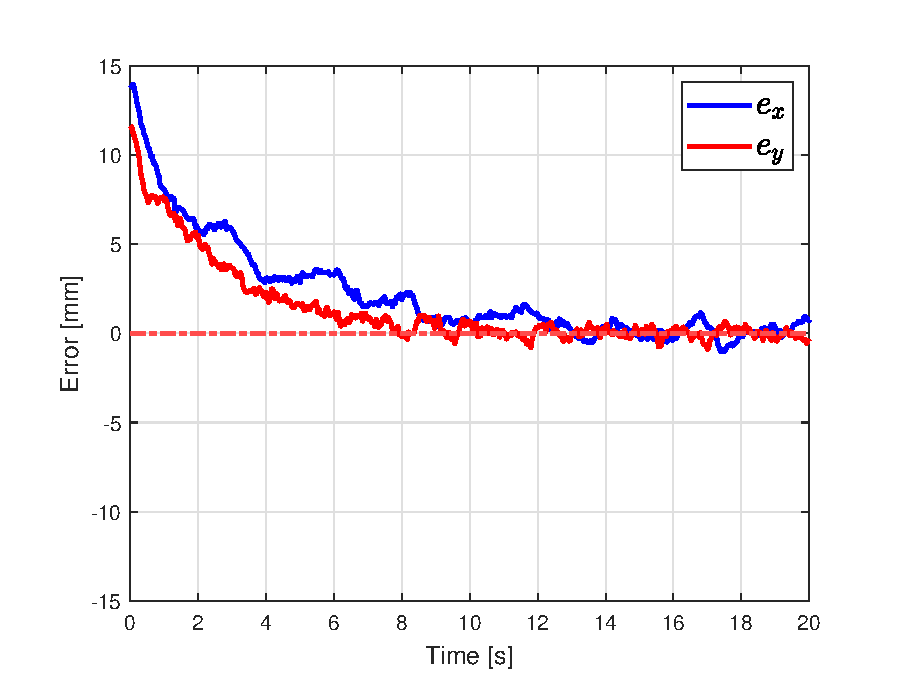
\includegraphics[width=\linewidth]{Figures/Chapter5/errorstepright.eps} 
    \caption{Error response in x and y-direction.Video provided at URL: \url{https://youtu.be/osywb0OYl7U}} 
    \label{fig5:errorswingright} 
       \end{minipage} 
    \begin{minipage}[b]{0.49\linewidth}
     \centering
    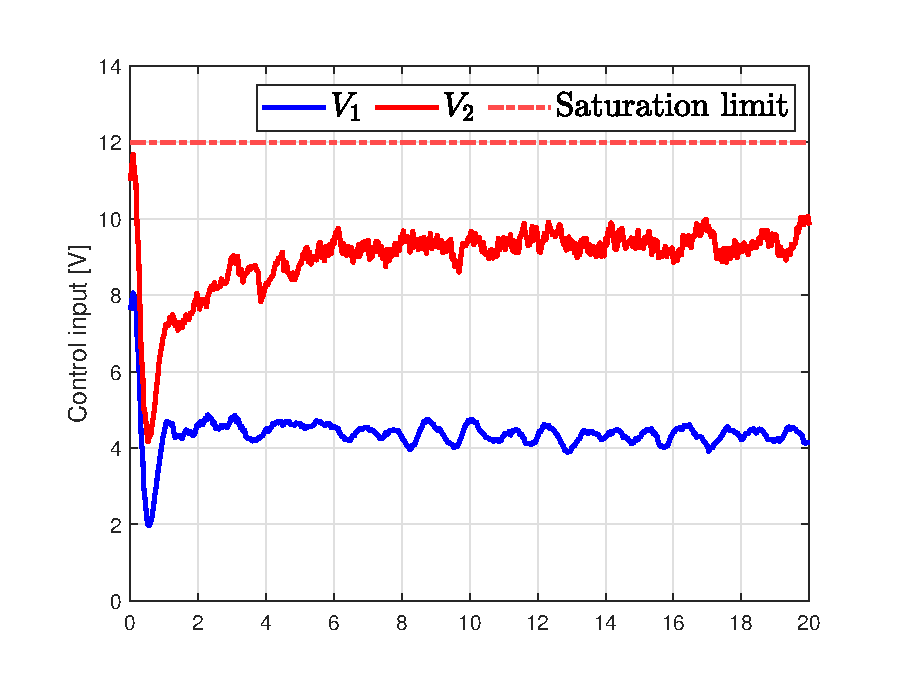
\includegraphics[width=\linewidth]{Figures/Chapter5/controlinputsteprightV.eps} 
    \caption{Volt control input signal to the air pumps.} 
    \vspace{12pt}
    \label{fig5:inputswingright} 
    \end{minipage} 
\end{figure}


\begin{figure}[H] 
    \begin{minipage}[b]{0.49\linewidth}
     \centering
    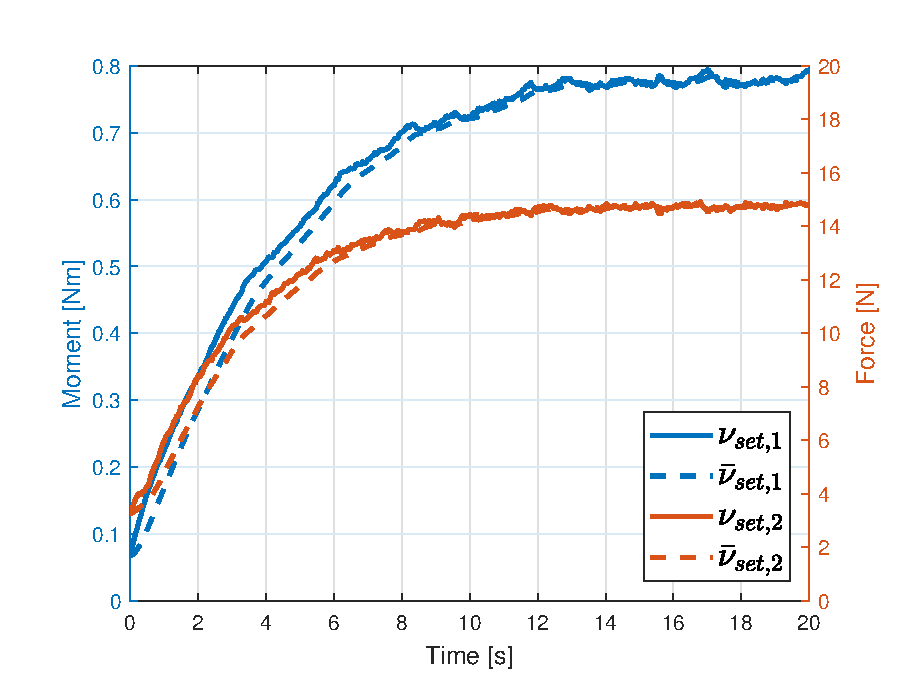
\includegraphics[width=\linewidth]{Figures/Chapter5/jacinputstepright.eps} 
    \caption{Input moment and force as determined by Jacobian controller. Solid line is unfiltered input, dotted line low-pass filtered. } 
    \label{fig5:nuright} 
       \end{minipage} 
    \begin{minipage}[b]{0.49\linewidth}
     \centering
    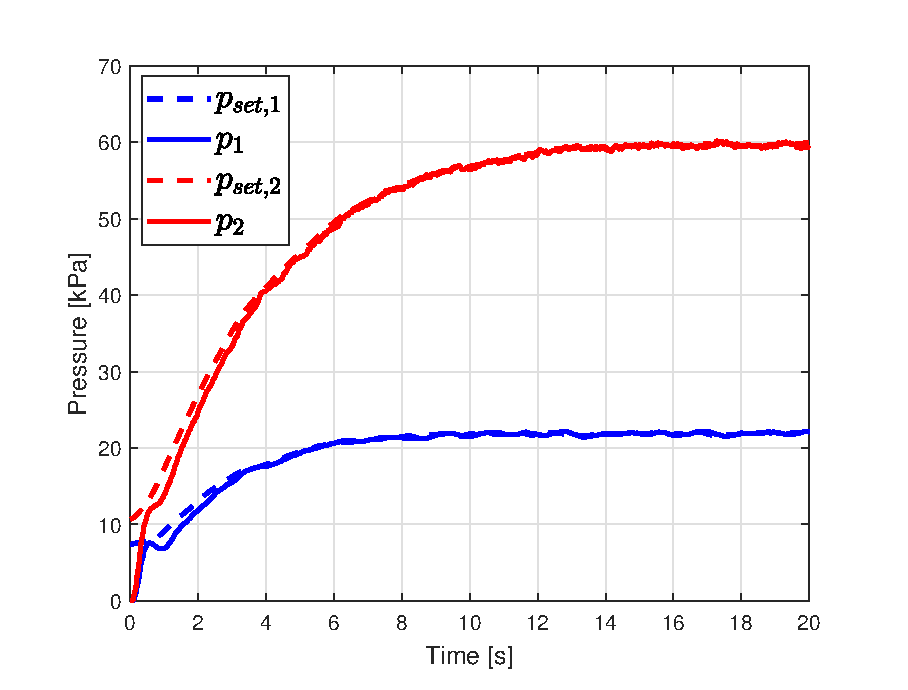
\includegraphics[width=\linewidth]{Figures/Chapter5/pressurestepright.eps} 
    \caption{Pressure response, dotted lines indicate reference pressure, solid lines are measured pressures.} 
    \label{fig5:pright} 
    \end{minipage} 
\end{figure}



Figure \ref{fig5:inputswingright} shows the Volt input to the air pumps. The observed response is similar to the previous set-point. The input during the first 1.5 seconds is initiated by a large initial error resulting in a high proportional action. After 1.5 seconds, the integrator action becomes dominant over the proportional gain. Eventually, the control input $V_1$ and $V_2$ stay around 4.3 V and 9.5 V, respectively. The maximum voltage is higher compared to the left set-point, as a higher bellow pressure needs to be attained. Figure \ref{fig3:pump_dynamics_adapted} in Chapter \ref{chap3} showed that for higher pressures the noise floor increases. The noise on the pressure readings affects the Volt input resulting in noise on input $V_2$. Furthermore, input $V_1$ is on the border of the static and dynamic friction region of the air pumps. This is causing the oscillations in input $V_1$. Both effects negatively affect the error response. Compared to the left set-point, the right error signal contains higher noise levels and oscillations. 




For both set-points, the RMS error is analyzed when the position error reaches steady-state. Therefore, the RMS error is calculated after 15 seconds for both set-points. The obtained error values are presented in Table \ref{tab:RMSerrors}. It can be seen that the RMS error for the right set-point is larger compared to the left set-point. The reason for this is the larger stiffness when bending to the right. This demands a larger pressure difference between both bellows. For one air pump, this implies a higher Volt input creating more noise on the pressure reading, while the other remains on the border region of static and dynamic friction.


\begin{table}[H]
    \centering
    \caption{RMS error after 15 seconds.}
    \begin{tabular}{|c|c|c|} \hline
     setpoint $[x,y]^\top$    & $e_{RMS,x}$ $mm$  &  $e_{RMS,y}$ $mm$  \\ \hline
    Left $r_{set}= [-0.014,0.082]^\top$     & 0.26034  & 0.22644 \\ \hline
    Right $r_{set}= [0.014,0.082]^\top$  &  0.32692&   0.26577\\ \hline
    \end{tabular}
    \label{tab:RMSerrors}
\end{table}



\subsection*{Closed-loop reference tracking in experiments}

To evaluate the performance of the controller during a reference tracking problem a similar ellipsoid reference signal is used. A small adaption is made regarding the first $t_1$ seconds in the y-direction reference profile. This is changed to,


\begin{equation}
    y_{ref} = \begin{cases} 
      \frac{(y_{off} - L) t}{t_1} + L&  t \leq t_1 \\
     (y_{off} +b) -  b \cos(2\pi \frac{t - t_1}{T_{ell}}) & t \leq T_{ell} + t_1 \\
     y_{off} & t > T_{ell} + t_1,
   \end{cases} 
\end{equation}

such that the y position reference linearly increases the first $t_1$ seconds. Furthermore, $T_{ell}$ which set the time to complete the ellipsoid is decreased from 400 seconds in simulation to 100 seconds for the experiments. An overview is presented in Table \ref{tab5:refparams}. 


\begin{table}[H]
    \centering
    \caption{Reference tracking parameters in experiments}
    \begin{tabular}{|c|c|} \hline
   \textbf{Parameter}  & \textbf{Value [unit]} \\ \hline
    $t_1$ &   15 [s]  \\ 
    $y_{off}$ & 0.074 [mm] \\
    $a$ & 13 [mm] \\
    $b$ & 7 [mm] \\
    $T_{ell}$ & 100 [s] \\ \hline
\end{tabular}
    \label{tab5:refparams}
\end{table}

The results of the above reference trajectory are plotted in Figure \ref{fig5:xyelips}. This figure shows the position in the x,y plane as a solid blue line, whereas the reference is plotted as a dotted black line. Additionally, green crosses mark the reference position at a given time, whereas red crosses mark the actual position at a given time. Overall, the tracking of the ellipsoid reference is improved compared to the results of \cite{berkers}. Furthermore, it can be seen that the actual position is lagging behind the reference position. Due to the discretization of the position data, it is hard to identify the exact delay in the system. When analyzing the data, an average delay of around 3.28 seconds is observed.  This delay is not constant during the entire reference path. As for the simulation, larger delays are observed for increasing pressure. Therefore, the cause of the delay is related to the dynamics of pumps. Feedforward control to the pumps would partly resolve these issues and therefore enhance the tracking performance of the system. Also, the filtering of the data causes delays in the system. However, these filtering effects are smaller than the influence of the pumps. 

\begin{figure}[H] 
    \begin{minipage}[b]{0.49\linewidth}
    \centering
    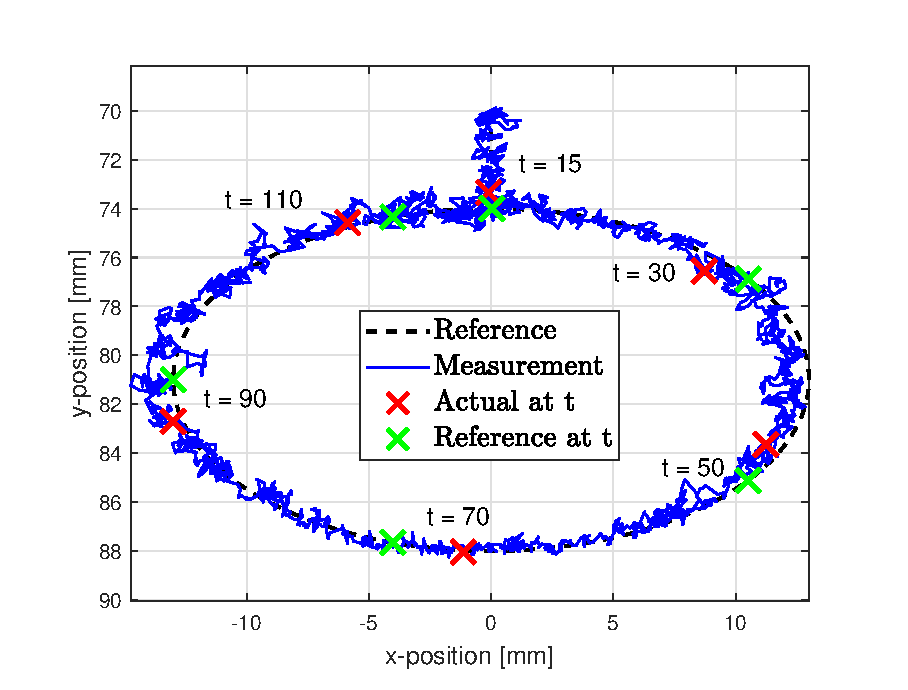
\includegraphics[width = \textwidth]{Figures/Chapter5/posellips.eps}
    \caption{Position in the x,y-plane for the ellipsoid reference path. Video provided at URL: \url{https://youtu.be/8hYWhlwnYkY}}
    \label{fig5:xyelips}
       \end{minipage} 
    \begin{minipage}[b]{0.49\linewidth}
    \centering
    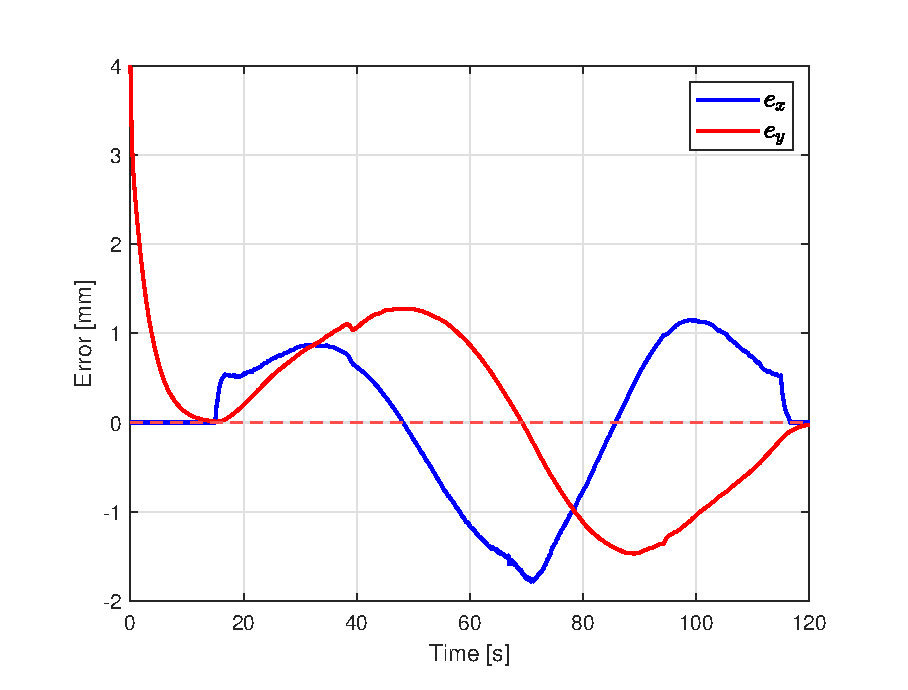
\includegraphics[width = \textwidth]{Figures/Chapter5/errorellips.eps}
    \caption{Error in the x and y-direction as a function of time for the ellipsoid reference path, accounted for 3.28 second delay.}
    %\hspace{10pt}
    \label{fig5:errorelips}
    \end{minipage} 
\end{figure}

Figure \ref{fig5:errorelips} shows the error in x and y-direction accounted for a delay of 3.28 seconds. The RMS error during reference tracking are $0.7926 \hspace{2pt} mm$ and $0.4044  \hspace{2pt} mm$ in x and y-direction, respectively. In the error response, an outlier is observed at 55 seconds. This might be caused by the vision system detecting an object other than the LED. 

Another observation is the noise in the error signal. There are two sources causing the noise on the position measurement. Firstly, the opening and closing of the air pump's diaphragms cause an inconsistent pressure flow into the system. This causes vibrations in the manipulator which translate itself to noise on the position measurement. To minimize the effect of the pumps on the position measurement, another method to inject air into the system is proposed. One of the options is a pressurized air vessel that is connected to a flow regulator. Ideally, this flow regulator can continuously regulate a valve position to control the airflow. 

The second reason is the vision system that is used for acquiring the position data. A major improvement would be a camera with a higher resolution. Such a camera is better at tracking the position as the discretization is smaller. Furthermore, increasing the update rate of the camera would be beneficial, as it would allow for better filtering of the data and a smaller delay. Given the current vision system, another color for the LED marker can improve the measurement. The yellow LED that is used in this experiment has almost the same hue value as the manipulator itself. Therefore the vision sometimes detects the manipulator instead of the LED. The software supplied with the vision system allows reducing this. However, changing the yellow LED with for instance a red LED would already improve the quality of the measurement.  

To improve tracking performance i.e. tracking speed and error reduction, feedforward actions can be implemented. This can be stiffness compensation added to the Jacobian controller. This stiffness compensation aids the controller in determining the reference force and moment for a given reference position. This could further be accompanied by a feedforward action on the pumps, to faster increase pressure. Both methods will decrease the effort of the integrator action, which is relatively slow. 


\begin{figure}[H]
    \centering
    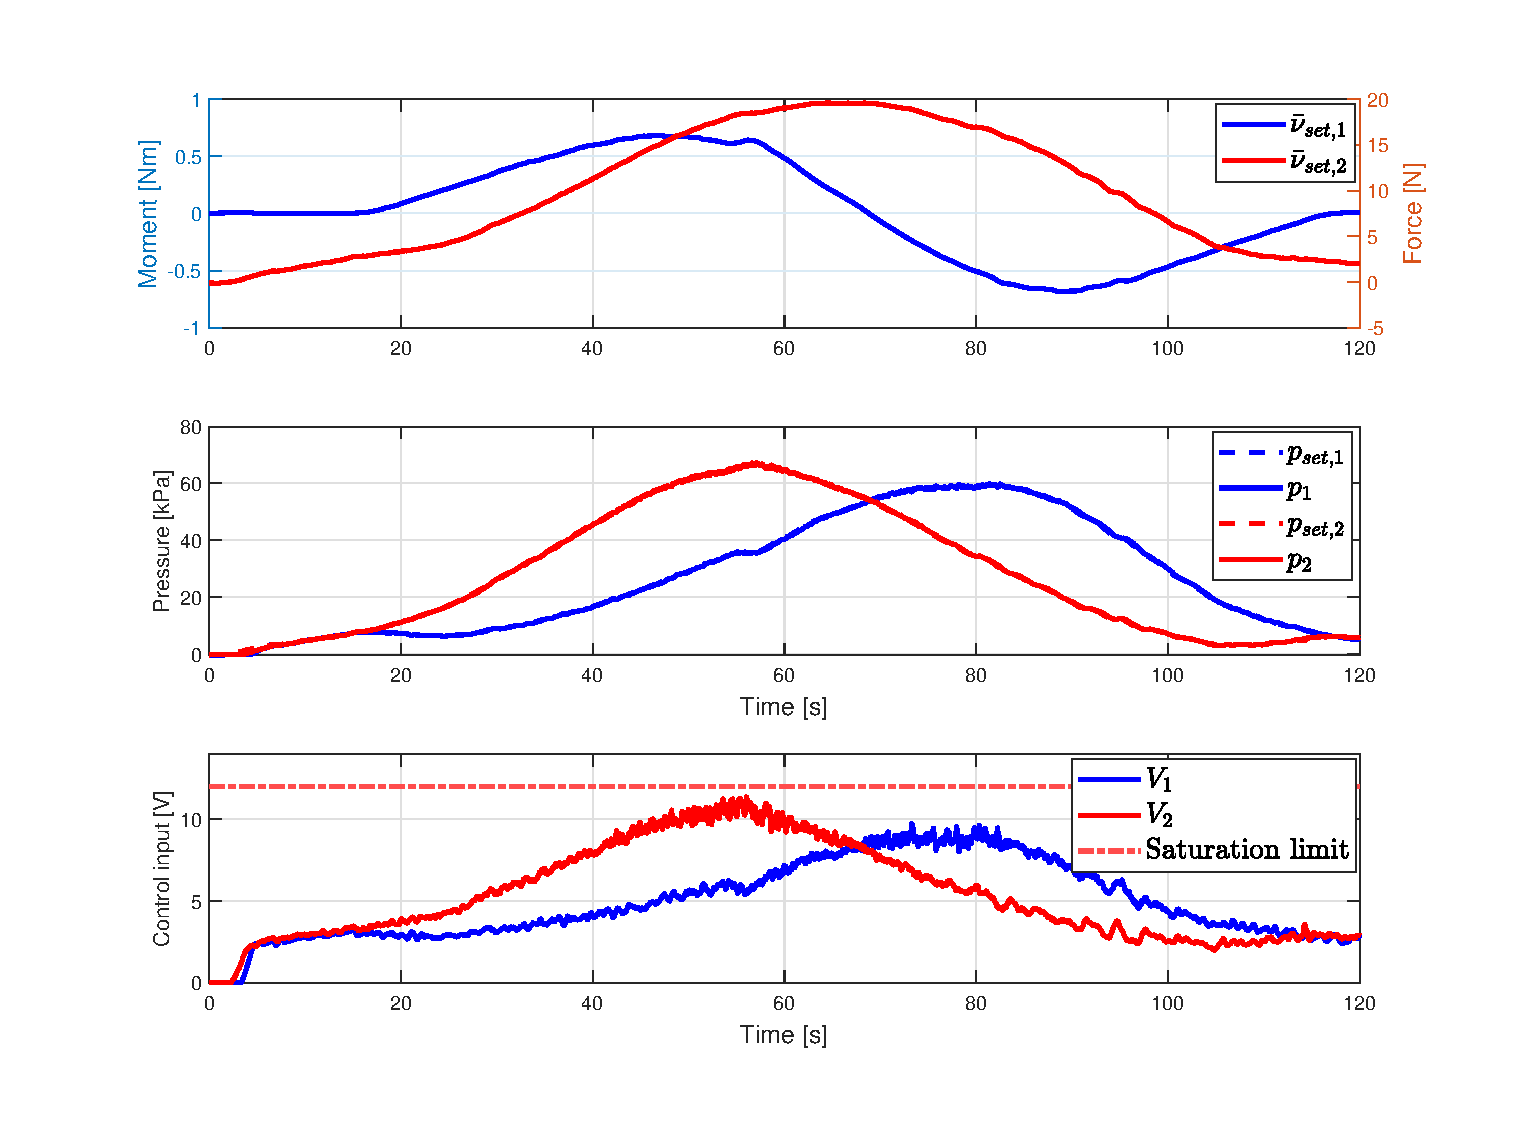
\includegraphics[width = 0.95\textwidth]{Figures/Chapter5/inputsellips.eps}
    \caption{\textbf{Top:} Control signal of model-based controller. \textbf{Middle:} Reference pressure and measured pressure. \textbf{Bottom:} Control input to the air pumps.}
    \label{fig5:controlellips}
\end{figure}


Figure \ref{fig5:controlellips}, shows the control input during the ellipsoid reference. The top figure displays the input as determined by the Jacobian controller. During the first $t_1$ seconds the moment is equal to zero, whereas the force is slowly increasing to induce the elongation. The moment then has two extrema at the time instance where x-displacement is required to be largest. The force is maximum, and the moment is near zero when the elongation of the manipulator is largest. The centre figure shows the pressure set-point and measured pressure over time. During the first half of the ellipsoid, a higher pressure $p_2$ is reached than $p_1$ in the second half. An explanation is the unsymmetrical material properties of the manipulator as concluded during the analysis of the step response. The bottom figure shows the Volt input to the air pumps. Near the saturation region, the control input to the air pumps has high-frequency noise. This is caused by higher noise levels on the pressure readings compared to lower pressures. Another notable phenomenon is the control input spikes occurring at 90 seconds. These are caused by a change in angular rate between the 3rd and 4th quadrant of the ellipsoid. At the switching plane between the 1st and 2nd quadrant, occurring at 40 seconds, this behaviour is not visible.




The pressure contour plot with timestamps is shown in Figure \ref{fig5:pressureellips}. Given the symmetrical ellipsoid reference, the pressure path is expected to be symmetrical as well. For relative low pressures, e.g. up to 50 kPa, this holds. However, for higher pressures, this symmetry argument does not hold. A major difference is that between 50 to 70 seconds the pressure is increasing, which is an active process. Between 70 and 90 seconds, the system is deflating. However, given that the tracking error in both regions is similar, the cause is most likely to be related to the not completely symmetrical stiffness properties.  





\begin{figure}[H] 
       \centering
    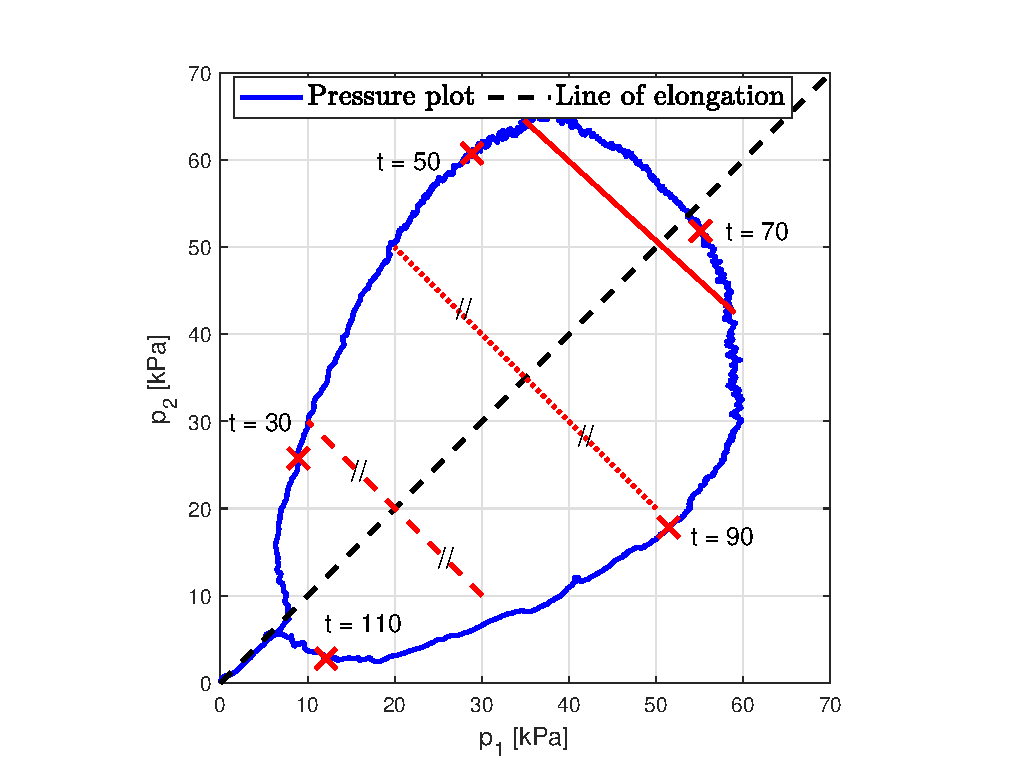
\includegraphics[width = 0.85\textwidth]{Figures/Chapter5/pcontourellips.eps}
    \caption{Contour plot of the bellow pressure $p_1$ and $p_2$, during ellipsoid reference tracking.}
    \label{fig5:pressureellips}
\end{figure}

\clearpage

\section{Model comparison to experimental results}

First of all, the model and experimental results show similar behaviour. The step responses are difficult to compare regarding settling times and controller gains as a different input mapping is used. However, the general behaviour of the controller is similar. First, a step like control input to the air pumps is initiated, causing the actuator to rapidly move to the reference direction. Then a dip in control input is observed. From that instant onwards the integrator gains cause the system to move to its desired position. In the experiments, a difference was observed for the mirrored set-points. This phenomenon is caused by non symmetric stiffness properties, while in simulation equal stiffness characteristics are assumed. 

Reference tracking in simulation and experiments also show equal characteristics. The largest difference is the time in which the ellipsoid reference path was tracked. The actual system was able to track the ellipse in 100 seconds with an RMS error of $0.7926 \hspace{2pt} mm$ and $0.4044 \hspace{2pt} mm$. For the model, the time to complete the ellipsoid was set to 400 seconds. In simulation, an RMS error of $e_x = 0.1489  \hspace{2pt} mm$ and $e_y = 0.0899 \hspace{2pt} mm$ was found. Both simulation and experiments show a time delay between the reference and actual position. The reason for this delay is the pump dynamics and low-pass filtering of the control input.



\subsection*{Summary}


In this chapter, the controller design and implementation are detailed. Based on the control layout the model-based controller and pressure controller are designed. The model-based controller uses the system's configuration dependent Jacobian to set the input force and moment. Via a mapping, this reference moment and force is translated to a set of reference pressures. Based on the reference pressure and current bellow pressure the Volt input to the air pumps is calculated. This controller is tested in simulation and experiments. In simulation, a step input is used to tune the controller. Then, a reference tracking problem is presented in simulation. The controller is also experimentally tested. To understand the experimental implementation, the setup and data acquisition is detailed. Again, a step response is used to tune the system in experiments. Then, a reference tracking problem in experiments is presented and the outcomes are analyzed. Lastly, a comparison between the model and experiments is provided. 



























